%% BU ECE template for MS thesis and PhD dissertation.
%%
%%==========================================================================%
%% MAIN PREAMBLE 
%%==========================================================================%
%\documentclass[12pt,letterpaper]{report}          % Single-sided printing for the library
%%\documentclass[12pt,twoside]{report} % Double-sided printing
%\usepackage[intlimits]{amsmath}
%\usepackage{amsfonts,amssymb}
%\DeclareSymbolFontAlphabet{\mathbb}{AMSb}
%%\usepackage{natbib}
%\usepackage{apalike}
%\usepackage{float}
%\usepackage[bf]{caption}       
%
%\usepackage{fancyhdr}
%%\usepackage{fancyheadings}
%\usepackage{fancybox}
%\usepackage{ifthen}
%\usepackage{bu_ece_thesis}
%\usepackage{url}
%\usepackage{lscape,afterpage}
%\usepackage{xspace}
%\usepackage{epstopdf} 
%\usepackage{subfig}
%%==========================================================================%
%%%% graphicx and pdf creation
%\usepackage{graphicx}
%\usepackage{appendix}
%%\usepackage{psfrag}
%%\DeclareGraphicsExtensions{.eps}   % extension for included graphics
%%\usepackage{thumbpdf}              % thumbnails for ps2pdf
%%\usepackage[ps2pdf,                % hyper-references for ps2pdf
%%bookmarks=true,%                   % generate bookmarks ...
%%bookmarksnumbered=true,%           % ... with numbers
%%hypertexnames=false,%              % needed for correct links to figures !!!
%%breaklinks=true,%                  % breaks lines, but links are very small
%%linkbordercolor={0 0 1},%          % blue frames around links
%%pdfborder={0 0 112.0}]{hyperref}%  % border-width of frames 
%%                                   % will be multiplied with 0.009 by ps2pdf
%%\hypersetup{
%	%  pdfauthor   = {Joe Graduate <joe.graduate@bu.edu>},
%	%  pdftitle    = {dissertation.pdf},
%	%  pdfsubject  = {doctoral dissertations},
%	%  pdfkeywords = {mathematics, science, technology},
%	%  pdfcreator  = {LaTeX with hyperref package},
%	%  pdfproducer = {dvips + ps2pdf}
%	%}
%%==========================================================================%
%% customized commands can be placed here
%%\newcommand{\figref}[1]{Figure~\ref{#1}}
%%\newcommand{\chapref}[1]{Chapter~\ref{#1}}
%%\newcommand{\latex}{\LaTeX\xspace}
%%==========================================================================%
%\usepackage[utf8]{inputenc} % set input encoding (not needed with XeLaTeX)
%\usepackage{amsmath,amssymb}
%\usepackage{mathtools}
%
%\usepackage{graphicx}
%\usepackage{glossaries}
%
%\usepackage{longtable}
%
%\usepackage{graphicx} % support the \includegraphics command and options
%
%% \usepackage[parfill]{parskip} % Activate to begin paragraphs with an empty line rather than an indent
%
%%%% PACKAGES
%
%\usepackage{varwidth} % must be loaded after array
%
%
%\usepackage{verbatim} % adds environment for commenting out blocks of text & for better verbatim
%
%\usepackage{array} % for defining a new column type
%
%% main git errors  handling https://www.javaprogramto.com/2021/11/error-failed-to-push-some-refs-to.html
%
%
%\newcommand{\numberset}[1]{\mathbb{#1}}
%\newcommand{\nat}{\numberset{N}}
%
%\DeclarePairedDelimiterX{\Set}[2]\{\}{%
%	\, #1 \;\delimsize\vert\; #2 \,
%}
%
%%%% Examples of Article customizations
%% These packages are optional, depending whether you want the features they provide.
%% See the LaTeX Companion or other references for full information.
%\renewcommand{\arraystretch}{2}
%
%\def\x#1{\texttt{\expandafter\string\csname#1\endcsname}&\expandafter$\csname#1\endcsname$}
%
%\newcommand{\stock}{\gets\mathrel{\mkern-2.4mu\mathop\square}}
%
%\let\mtproforall\forall % just for the comparison
%\let\mtproexists\exists % just for the comparison
%
%\DeclareSymbolFont{CMsymbols}{OMS}{cmsy}{m}{n}
%\SetSymbolFont{CMsymbols}{bold}{OMS}{cmsy}{b}{n}
%\DeclareMathSymbol{\forall}{\mathord}{CMsymbols}{"38}
%\DeclareMathSymbol{\exists}{\mathord}{CMsymbols}{"39}
%
%\makeatletter
%\providecommand*{\Dashv}{%
%	\mathrel{%
%		\mathpalette\@Dashv\vDash
%	}%
%}
%\newcommand*{\@Dashv}[2]{%
%	\reflectbox{$\m@th#1#2$}%
%}
%\makeatother
%
%
%\newcolumntype{L}[1]{>{\flushleft\arraybackslash}p{#1}}
%%==========================================================================%
%% BEGIN
%%==========================================================================%
%\begin{document}
%	
%	% The preliminary pages
%	% This file contains all the necessary setup and commands to create
% the preliminary pages according to the buthesis.sty option.

\title{Eindverslag tinlab Advanced Algorthms}

\author{Galvin Bartes}

% Type of document prepared for this degree:
%   1 = Master of Science thesis,
%   2 = Doctor of Philosophy dissertation.
\degree=2

\prevdegrees{B.S., Hogeschool Rotterdam University, 2022}

\department{Departement Communicatie- Media- en Informatietechnologie}

% Degree year is the year the diploma is expected, and defense year is
% the year the dissertation is written up and defended. Often, these
% will be the same, except for January graduation, when your defense
% will be in the fall of year X, and your graduation will be in
% January of year X+1
\defenseyear{2022}
\degreeyear{2022}

% For each reader, specify appropriate label {First, Second, Third},
% then name, and title. IMPORTANT: The title should be:
%   "Professor of Electrical and Computer Engineering",
% or similar, but it MUST NOT be:
%   Professor, Department of Electrical and Computer Engineering"
% or you will be asked to reprint and get new signatures.
% Warning: If you have more than five readers you are out of luck,
% because it will overflow to a new page. You may try to put part of
% the title in with the name.
\reader{First}{Remco M. Last, PhD}{Professor of Electrical and Computer Engineering}
\reader{Second}{Mostafa M. Last}{Associate Professor of \ldots}
\reader{Third}{Marco M. Last}{Assistant Professor of \ldots}

% The Major Professor is the same as the first reader, but must be
% specified again for the abstract page. Up to 4 Major Professors
% (advisors) can be defined. 
\numadvisors=2
\majorprof{First Wessel. Oele, PhD}{{Professor of Electrical and Computer Engineering\\Secondary appointment}}
\majorprofb{First M. Last, PhD}{{Professor of Computer Science}}
%\majorprofc{First Nadine. van Dormolen, PhD}{{Professor of Astronomy}}
%\majorprofd{First M. Last, PhD}{{Professor of Biomedical Engineering}}

%%%%%%%%%%%%%%%%%%%%%%%%%%%%%%%%%%%%%%%%%%%%%%%%%%%%%%%%%%%%%%%%  

%                       PRELIMINARY PAGES
% According to the BU guide the preliminary pages consist of:
% title, copyright (optional), approval,  acknowledgments (opt.),
% abstract, preface (opt.), Table of contents, List of tables (if
% any), List of illustrations (if any). The \tableofcontents,
% \listoffigures, and \listoftables commands can be used in the
% appropriate places. For other things like preface, do it manually
% with something like \newpage\section*{Preface}.

% This is an additional page to print a boxed-in title, author name and
% degree statement so that they are visible through the opening in BU
% covers used for reports. This makes a nicely bound copy. Uncomment only
% if you are printing a hardcopy for such covers. Leave commented out
% when producing PDF for library submission.
%\buecethesistitleboxpage

% Make the titlepage based on the above information.  If you need
% something special and can't use the standard form, you can specify
% the exact text of the titlepage yourself.  Put it in a titlepage
% environment and leave blank lines where you want vertical space.
% The spaces will be adjusted to fill the entire page.
\maketitle
\cleardoublepage

% The copyright page is blank except for the notice at the bottom. You
% must provide your name in capitals.
\copyrightpage
\cleardoublepage

% Now include the approval page based on the readers information
% Once the approval page is approved by the Mugar Library staff, please
% comment out the "\approvalpagewithcomment" line and uncomment "\approvalpage"
\approvalpagewithcomment
%\approvalpage
\cleardoublepage

% Here goes your favorite quote. This page is optional.
\newpage
%\thispagestyle{empty}
\phantom{.}
\vspace{4in}

\begin{singlespace}
\begin{quote}
  \textit{Facilis descensus Averni;}\\
  \textit{Noctes atque dies patet atri janua Ditis;}\\*
  \textit{Sed revocare gradum, superasque evadere ad auras,}\\
  \textit{Hoc opus, hic labor est.}\hfill{Virgil (from Don's thesis!)}
\end{quote}
\end{singlespace}

% \vspace{0.7in}
%
% \noindent
% [The descent to Avernus is easy; the gate of Pluto stands open night
% and day; but to retrace one's steps and return to the upper air, that
% is the toil, that the difficulty.]

\cleardoublepage

% The acknowledgment page should go here. Use something like
% \newpage\section*{Acknowledgments} followed by your text.
\newpage
\section*{\centerline{Acknowledgments}}
Het is geweldig om dit vak te herkansing met twee fantastische collega's

\vskip 1in

\noindent
Galvin Bartes\\
Student\\
 

\noindent
Tycho\\
Student\\

\noindent
Koosha\\
Student\\
CMI



\cleardoublepage

% The abstractpage environment sets up everything on the page except
% the text itself.  The title and other header material are put at the
% top of the page, and the supervisors are listed at the bottom.  A
% new page is begun both before and after.  Of course, an abstract may
% be more than one page itself.  If you need more control over the
% format of the page, you can use the abstract environment, which puts
% the word "Abstract" at the beginning and single spaces its text.

\begin{abstractpage}
% ABSTRACT

Het ministerie van verkeer en Waterstaat wil in het kader van het klimaatakkoord en onderzoek laten uitvoeren naar de staat van het sluizenpark in Nederland. Het onderzoek moet zich richten op het ontwerpen en ontwikkelen van een geautomatiseerd sluismodel dat geschikt is voor een brede toepassing. In het onderzoek moet naar voren komen wat de huidige staat is van de sluizen met oog op veiligheid, efficiëntie, capaciteit, onderhoud, duurzaamheid en automatisering. Het onderzoek geeft aan hoe een volledig model worden opgeleverd opdat ontwerp van verschillend volledig geautomatiseerde sluizen in de toekomst geautomatiseerd kunnen worden.  

managementsamenvatting
Inleiding
aanleiding, context, hoofdvraag van het rapport. Is de aanpak van het ziekteverzuim effectief?

Doelen van de aanpak ziekteverzuim
Wat is de gewenste situatie?
Wat is de huidige situatie?

Toetsingscriteria
Hoe is de huidige situatie getoetst?
Criterium 1
Criterium 2

Balans 
hoe zwaar wegen de uitkomsten

Conclusie
Wat is dus, gezien  het bovenstaande, het antwoord op de hoofdvraag van het rapport?
\end{abstractpage}
\cleardoublepage

% Now you can include a preface. Again, use something like
% \newpage\section*{Preface} followed by your text

% Table of contents comes after preface
\tableofcontents
\cleardoublepage

% If you do not have tables, comment out the following lines
\newpage
\listoftables
\cleardoublepage

% If you have figures, uncomment the following line
\newpage
\listoffigures
\cleardoublepage

% List of Abbrevs is NOT optional (Martha Wellman likes all abbrevs listed)
\chapter*{List of Abbreviations}

{\bf The list below must be in alphabetical order as per BU library instructions or it will be returned to you for re-ordering.}

\begin{center}
  \begin{tabular}{lll}
    \hspace*{2em} & \hspace*{1in} & \hspace*{4.5in} \\
    CAD  & \dotfill & Computer-Aided Design \\
    CO   & \dotfill & Cytochrome Oxidase \\
    DOG  & \dotfill & Difference Of Gaussian (distributions) \\
    FWHM & \dotfill & Full-Width at Half Maximum \\
    LGN  & \dotfill & Lateral Geniculate Nucleus \\
    ODC  & \dotfill & Ocular Dominance Column \\
    PDF  & \dotfill & Probability Distribution Function \\
    $\mathbb{R}^{2}$  & \dotfill & the Real plane \\
  \end{tabular}
\end{center}
\cleardoublepage

% END OF THE PRELIMINARY PAGES

\newpage
\endofprelim
        
%	\cleardoublepage
%	
%	% -------------------------------------
%	% CHAPTER 1: INTRODUCTION
%	% -------------------------------------
%	\newpage
\section{Inleiding}
In deze case study wordt %insert inleiding hier

\subsubsection{Algemeen}

Het ministerie van verkeer en Waterstaat wil in het kader van het klimaatakkoord en onderzoek laten uitvoeren naar de staat van het sluizenpark in Nederland. Het onderzoek moet zich richten op het ontwerpen en ontwikkelen van een geautomatiseerd sluismodel dat geschikt is voor een brede toepassing. In het onderzoek moet naar voren komen wat de huidige staat is van de sluizen met oog op veiligheid, efficiëntie, capaciteit, onderhoud, duurzaamheid en automatisering. Het onderzoek geeft aan hoe een volledig model worden opgeleverd opdat ontwerp van verschillend volledig geautomatiseerde sluizen in de toekomst geautomatiseerd kunnen worden.  

\subsubsection{Recente ontwikkelingen op het gebied van sluisautomatisering}

Het ministerie van verkeer en Waterstaat wil in het kader van het klimaatakkoord en onderzoek laten uitvoeren naar de staat van het sluizenpark in Nederland. Het onderzoek moet zich richten op het ontwerpen en ontwikkelen van een geautomatiseerd sluismodel dat geschikt is voor een brede toepassing. In het onderzoek moet naar voren komen wat de huidige staat is van de sluizen met oog op veiligheid, efficiëntie, capaciteit, onderhoud, duurzaamheid en automatisering. Het onderzoek geeft aan hoe een volledig model worden opgeleverd opdat ontwerp van verschillend volledig geautomatiseerde sluizen in de toekomst geautomatiseerd kunnen worden.  
\subsubsection{Wat is een sluis}

\subsubsection{Wat worrdt er omschreven en wat is er geleerd}

\subsubsection{Wat is uppaal}

Wat is Uppaal
Uppaal is an integrated tool environment for modeling, simulation and verification of real-time systems, developed jointly by Basic Research in Computer Science at Aalborg University in Denmark and the Department of Information Technology at Uppsala University in Sweden. It is appropriate for systems that can be modeled as a collection of non-deterministic processes with finite control structure and real-valued clocks, communicating through channels or shared variables [WPD94, LPW97b]. Typical application areas include real-time controllers and communication protocols in particular, those where timing aspects are critical.


model checking

Wat is statistical model checking?
Dit verwijst naar verschillende technieken dfie worden gebruikt voor de monitoring van een systeem. Daarbij wordt vooral gelet op een specifieke eigenschap. Met de resultaten van de statsitieken wordt de juistheid van een ontwerp beoordeeld. Statistisch model checking wordt onder andere toegepast in systeembiologie, software engineering en industriele toepassingen.
https://www-verimag.imag.fr/Statistical-Model-Checking-814.html?lang=en#:~:text=Statistical%20Model%20Checking%20(SMC)%20is,from%20state%20space%20explosion%20issues.

Model Checking (MC) [BK08,CGP99] is a widely recognized approach to guarantee correctness of a system. The technique relies on algorithms that check whether all executions of a system satisfy some properties stated in a specification logic. If this is the case, then the system is correct, else a bug is reported.
First implementations of model checking suffered from so-called state space explosion problems and could only be applied to small academic models. New techniques build on symbolic data structures and/or heuristics that make them capable of analyzing large-size systems that are part of our daily life
lassical model checking techniques are Boolean (either the system satisfies a property or it does not). Unfortunately such a view is extremely sensitive to changes made in the design and is not able to quantify their impacts (both minor and major changes may reverse the verification outcome).  This view is now obsolete: the designers need a finer analysis that allows to quantify the impacts of any change in the design. This has motivated the development of a series of new techniques (under the name of Probabilistic Model Checking) and tools [PRISM,BK08] capable of quantifying the likelihood for a system (whose behaviors naturally depend on stochastic information) to satisfy some property.  Adding explicitly rich features (e.g., real time) in specifications is also needed. Indeed, in many situations it is not enough to know whether something will or will not happen; rather, one needs to have a precise estimate of the time when some situation will arise. This motivated the creation of a number of new techniques under the name of timed model checking. 
The problem with MC-based approaches is that even though heuristics exist (partial order, symbolic approach, BDDs, etc.), they still suffer from the state-space explosion problem. This is especially the case when the system is obtained as the combination of several subsystems. Moreover, when moving to rich systems such as those with real time features, most of the model checking problems become undecidable.

 \cite{inriaStatsMoodCheck}
 \cite{ buddeModelChecker}
 \cite{AGHASuervey }
 

Waarom gebruiken we statistisch model checking?
To overcome the above difficulties we propose to work with Statistical Model Checking [KZHHJ09,You05,You06,SVA04,SVA05,SVA05b] an approach that has recently been proposed as an alternative to avoid an exhaustive exploration of the state-space of the model. The core idea of the approach is to conduct some simulations of the system, monitor them, and then use results from the statistic area (including sequential hypothesis testing or Monte Carlo simulation) in order to decide whether the system satisfies the property or not with some degree of confidence. By nature, SMC is a compromise between testing and classical model checking techniques. Simulation-based methods are known to be far less memory and time intensive than exhaustive ones, and are oftentimes the only option. 
https://project.inria.fr/plasma-lab/statistical-model-checking/

Alternatief
Alternatieven voor Uppaal zijn Asynchronous Events,Vesta en MRMC.
%%%%%%%%%%%%%%%%%%%%%%%%%%%%%%%%%%%%%%%%%%%%%%%%%%%%%%%%%%%%%%%%%

\subsubsection{Probleemanalyse}

Na grondige analyse van het Nederlandse sluizenpark is gebleken dat renovatie van een groot aantal sluizen noodzakelijk is.  Uit een eerste verkenning is gebleken  dat het gecombineerd renoveren en automatiseren van het Nederlandsesluizenpark een aanzienlijke verbetering kan opleveren t.a.v. 
Op  het  ministerie  van  infrastructuur  enwaterstaat is helaas onvoldoende kennis van ict en systemen aanwezig om eenen ander uit te voeren 

\subsubsection{Waarom nu}
In  het  kader  van  het  onlangs  afgesloten  klimaatakkoord  heeft  de  Nederlandseoverheid  daarom  besloten  over  te  gaan  tot  een  ingrijpende  renovatie  van  dediverse  sluizen  die  ons  land  rijk  is.     

\subsubsection{Gewenst resultaat }


Wij vragen u een model (of een onderling samenhangend aantal modellen)aan  te  leveren,  opdat  ontwerpen  van  verschillende,  volledig  geautomatiseerdesluizen in de toekomst gerealiseerd kunnen worden. 
Zoals  gesteld  in  de  brief  is  het  de  bedoeling  dat  een  sluis  gemodelleerd  wordten  dat  bewezen  kan  worden  dat  de  te  bouwen  sluis  een  aantal  eigenschappenbezit.  

\subsubsection{Scope}

He gaat om het simuleren van een geautomatiseerde sluis. Wat voor type sluis wordt niet gemeld en ook niet uit welke onderdelen. Belangrijk is dat het model werkt en dat het voldoet aan de eisen die gebaseerd zijn op basis van literatuuronderzoek, observatie, interviews, brainstorming of een andere vorm van requirements elicitation.

\subsubsection{Onderzoeksvragen }

Hoe kan een geautomatiseerde sluis worden gemodeleerd met oog op ontwikkel- en onderhoudskosten,veiligheid, efficientie en capaciteit





\begin{enumerate}

	\item Welke requirements en kwaliteitseisen komen naar voren bij de analyse van een rampenonderzoek
	\item Welke veiligheidseisen er zijn voor sluizen in nederland. 
	\item Hoe kan in uppaal  een model worden getest dat voldoet aan de requirements/eisen volgens het rampenonderzoek?
\end{enumerate}

%%%%%%%%%%%%%%%%%%%%%%%%%%%%%%%%%%%%%%%%%%%%%%%%%%%%%%%%%%%%%%%%%


\subsubsection{Design goals}
Het systeem moet minimaal aan de volgende prestatie eisen voldoen 

\begin{enumerate}
	\item  
	\begin{enumerate}
		\item Requirements gebaseerd op rampenanalyse
	\end{enumerate}
	\item Data
	\begin{enumerate}
		\item Model testbaar in upaal
	\end{enumerate}
	
\end{enumerate}

%%%%%%%%%%%%%%%%%%%%%%%%%%%%%%%%%%%%%%%%%%%%%%%%%%%%%%%%%%%%%%%%%
\subsubsection{Welke aanpak is gekozen en welke studies liggen hieraan ten grondslag?}
https://link.springer.com/article/10.1007/s10626-020-00314-0

\subsubsection{Leeswijzer}
In  de methodologie wordt de lezer uitgelegd met welke methoden de onderzoeksvragen zijn beantwoord. In het hoofdstuk Onderzoek worden alle resultaten behandeld die naar voren zijn gekomen bij het deskresearch. De analyse van de verzamelde data wordt gedaan in het hoofdstuk analyse. Hierin wordt behandeld zoekopdracht naar IoT cloud platforms, feature extractie, prijs-berekening en prijs-feature vergelijking. In het ontwerp komen de uml diagrammen en systeemschetsen naar voren. In de  de hoofdstukken Prototype, IoT cloud en Firmware wordt de implementatie behandeld van het IoT cloud platform in een bestaand project.

%%%%%%%%%%%%%%%%%%%%%%%%%%%%%%%%%%%%%%%%%%%%%%%%%%%%%%%%%%%%%%%%%



%	\input{Methoden} %(verplicht) hoofdverslag
%\hoofdstuk{methoden}
 
%	\cleardoublepage
%	
%	% -------------------------------------
%	% CHAPTER 2: THE BODY OF THESIS
%	% -------------------------------------
%	\graphicspath{{2_Body/Figures/}}




\chapter{Methodologie}
\label{chapter:body}
\thispagestyle{myheadings}




\chapter{Theoretisch kader}
\subsection{MODE CONFUSION }
Mode confusion tredd op als gepbserveerd gedrag van een technisch systeem niet past in het gedragspatroon dat de gebruiker in zijn beeldvorming heeft  en ook niet met voorstellingsvermogen kan bevatten.
\subsection{Wat is automatiseringsparadox}
Gemak dient de mens. Als er veel energie wordt gestoken in de ontwikkeling van hulmiddelen die taken van werknemers overemen heeft dat tot resultaat dat veel productieprocessen worden geautomatiseerd. De vraag is dan of vanuit mechnisch wereldpunt de robot niet de rol van de mens overneemt en of de mens nog de kwaliteiten heeft om het werk zelf te doen.

\url{https://www.dalton.nl/literatuur/item/252-de-automatiseringsparadox}
\url{https://www.debicker.eu/de-automatiseringsparadox/}
\url{https://vse.nl/de-paradox-van-de-industriele-automatisering/}
\url{https://automatie-pma.com/nieuws/industriele-automatiseringsparadox}
\url{https://blog.xot.nl/2016/11/21/slimme-apparaten-maken-ons-dom-en-kwetsbaar/index.html}

\subsection{Wat is een model}
\subsubsection{Conceptueel model}
Om duding te geven aan het grote plaatsje
\subsubsection{in vivo model}
Levende organismendie in de werkelijkheid of in een laboriatrum vergelijkbare eigenschappen bezitten als bestaande fenomenen in de werkeljkheid. Deze objecten zijn vergelijkbaar met werkelijkobjecten en geven vergelijkbare resultaten
\subsubsection{in vitro model}
Een model dat dezelfde condities biedt  buiten het onderzoeksobject om, maar is voldoende vergelijkbaar om vergelijkbare processen te simuleren.
Zowel invivo als in vitro modellen zijn beperkt door de materialen die beschikbaar ijn voor onderzoek en de arbeidsomstandigheden waaronder ze worden gebruikt. Desondanks zijn het geen werkelijke natuurlijke modellen dus vvoor een onderzoek kan boedt het geen volledige uitsluitsel.
\subsubsection{In silicio model}
Ee veelzijdig object. Het verwijst naar simulaties die gebruik maken van wiskundige modellen in computer,een zijn dus afhankelijk van silicone chips. In silico model analyseert  wiskundige vergelijkingen om resultaten te geven onder bepaalde omstandigheden. Deze vergelijkingen vertellen iets over de correlatie van verschillende objecten van een wetenschappelijk onderzoek. OM deze modellen te kunnen gebruiken is het noodzakelijk te omschrijven waat de fenomenen in kwestie van onderzoek zijn door middel van getallen. Kwanttitatieve relaties kunnen worden geintegreerd in het model en waar deze relaties complex zijn is een computer noodzakelijk deze op telossen. Vaak worden hierbij verschillende mechanismen gebruikt. Als je bijvoorbeeld de prijsontwikkeling van een marsreep in kaart wilt brengen.
\subsubsection{in simulacra model}

\subsection{World and machine samenvatting}
Waarom zijn wij engineers? Omdat we bruikbare apparaten willen laten functioneren in de wereld waarin we leven. Dat doen we door de machine te beschrijven en deze beschrijving van instructies bieden we aan onze computer opdat deze als de attribuut en gedragingen uitleest zoals wij die hebben omschreven. Dit alles op basis van theoretische funderingen en praktisch inzicht. 

Het doel van een machine is om te worden geinstalleerd en te worden gebruikt. De eisen die we stellen zitten in de omgeving en in de wereld en de machine is slechts de oplossing die we bedenken om aan een eis te voldoen. 

De relatie machine-wereld world gecategoriseerd in: 

Het modelleer aspect: waar een machine de wereld simuleert 

Het interface aspect: waar er fysieke interactie is tussen de machine en de wereld 

Het engineering aspect: waar de machine zich gedraagt als een controlemotor gebruikmakend van de gedragingen van de omgeving in de wereld 

Het probleem aspect: waar de omgeving in de wereld en de omvang van het probleem invloed heeft op de machine en de oplossing 

Het modelleer  of simulatie aspect over een deel van de wereld. Er zijn data,object en proces modellen. Het doel van een model is toegang te geven tot informatie over die wereld. Door het opvangen van statische weergaven en gebeurtenissen kunnen wij deze gebruiken van opgeslagen informatie die we kunnen hergebruiken. Een model kan bruikbare informatie bevatten omdat zowel het model als de wereld warin het model zich bevind gemeenschappelijke omschrijvingen hebben die waar zijn voor zwel het model als voor de wereld. Daarbij moet gesteld worden dat de interpretatie van een model verschilt met een interpretatie van de wereld. 

Omdat zowel de wereld als de machine fysieke realiteiten zijn an niet slechts abstracties, zijn de gemeenschappelijke beschrijvingen slechts een deel van de werkelijheid van beide objecten. For elk object zijn er meerdere beschrijvingen. Toch maken niet alle omschrijvingen deel uit van het getoonde reportoire. Zoals niet alle eigenschappen van een boek; meer dan een auteur, pseudoniemen, een onderdeel van een reeks, een gerevisiteerde versie, worden gereflecteerd in een database.  

Het interface aspect. Een machine kan een probleem in de wereld oplossen als de wereld en de machine phenomena kunnen uitwisselen. Maar de participatie is niet symmetrisch: een status kan als phenomena worden uitgewisseld maar slechts een partij kan er invloed op uitoefenen maar beiden kunnen dezelfde status signaleren. 

Het engineering aspect gaat over requirements, specificaties, en programma’s. Requirements hebben betrekking op phenomena in de wereld. Een programma heeft alleen betrekking tot de machinale phenomena. Het doel van programma’s is om eigenschappen en gedragingen te omschrijven van de machine ten behoeve van de gebruiker. Tussen de requirements en de programma’s zitten de specificaties. Omdat programma’s dan wel beschrijvingen zijn van een gewenste machine, maar dat moeten beschrijvingen zijn van de  machines  die de computers kunnen uitvoeren zodanig dat de computer deze beschrijvingen ook zo kan interpreteren. De engineer moet  de eigenschappen van de wereld kennen en begrijpen en deze eigenschappen manipuleren en laten werken met als doel het dienen van het systeem. 

Het probleem aspect. Het onderscheid tussen specificatie en implementatie. Het probleem zit in de relatie van de machine en de wereld. De machine brengt de oplossing maar het probleem zit in de wereld. Een vertoog over een probleem moet dus gaan over de wereld en over de opvatting die de gebruiker heeft in de wereld. Omdat de wereld veelzijdig is moeten we ervan uit gaan dat er verschillende soorten problemen zijn. Een realistisch probleem wordt dus niet opgelost met een simpele hiërarchische structurele aanpak en een homogene decompositie maar met een paralleele structurele oplossing waar beide kanten van het probleem worden opgelost. 



Ontkenningen 

We hebben als engineers de taak om een machine te bouwen aan de hand van de specificaties opgeleverd door de opdrachtgever. Een engineer heeft niet als taak de fitheid voor een doeleind te onderzoeken, maar wel de haalbaarheid naar een doeleind aan de hand van kennis, tijd, resources, budget en ontwikkelmethodiek. Daaruit komt naar voren dat een engineer zich richt op: elicitation (schetsen van een requirement), description (omschrijving) en analyse van de requirements waaraan het systeem moet voldoen. Vertaalt naar de volgende vragen: Wat is precies de klantwens?  Wat is de precieze omschrijving van het probleem? Voor welke doelen wordt het systeem gebouwd? Welke functies moet het systeem hebben? 

Denial by hacking: obsessief bezig zijn met een systeem omdat het de gebruiker veel macht geeft. Een uitgebreidheid van een systeem zorgt er soms voor dat mensen niet meer geprikkeld zijn na te denken over probleemstellingen, domein beschrijvingen en analyse. 

Denial by a abstraction. Wiskundige benaderingen van werkelijke problemen is  een belangrijke intellectuele strategie om problemen te formuleren. Een software ontwikkelaar moet een probleem kunnen omschrijven in zo min mogelijk woorden, maar de complexiteit ligt in de oplossing. 

Denial by vagueness. De vaagheid van een omschrijving is terug te vinden in: 

Von Neumann’s principe 

Principe van reductionisme 

Shanley principe 

Montaingnes’s principe 

Von Neumand principe 

Voor een vocabulair  moet een grondslag zijn ontwikkeld waarmee gesproken kan worden over de wereld en de machine. Belangrijke phenomenen moeten geindtifieerd worden, door middel van een grondregel  of ‘herkenningsregel’ moet een fenomeen worden herkend, en vervolgens het fenomeen een formele term geven die gebruikt wordt als duiding van een bepaalde omschrijving. Dan moet voor de formele term een symbool gevonden worden. Samen vormen de grondregel en het symbool een designatie. 

Principe van reductionisme 

Simpelweg het openbreken van termen met een weerlegbare definitie totdat alle begrippen die worden gebruikt om iets te duiden  niet meer te herconstrueren zijn in hun definitie. 

Shanley principe 

Er bestaan volgens dit principe geen scherpe verdelingen in de wereld zoals wetenschappers soms denken. Een strenge opvatting over de wereld waarin een individu geclassificeerd kan worden als een onsamenhangend geheel. Maar dat is slechts een opname van een beeld. De werkelijkheid staat soms toe dat een elementair individueel object in verschillende classificaties verschillende getypeerd kan worden in een andere setting of view. 

Montaignes principe 

De incative mood; gaat over wat we beweren waar te zijn. 

De optitative mood; gaat over wat we willen dat waar is 
\subsection{SIX Variable model}
Optitatieve statements omschrijven de omgeving zoals we het willen zien vanwege de machine. 

Indicatieve statements omschrijven de omgeving zoals deze is los van de machine. 

Een requirement is een optitatief statement omdat ten doel heeft om de klantwens uit te drukken in een softwareontwikkel project. 

Domein kennis bestaut uit indicatieve uitspraken die vanuit het oogpunt van software ontwikkeling relevant zijn. 

Een specificatie is een optitatief statement met als doel direct implementeerbaar te zijn en ter verondersteuning van het natreven vande requirements. 

Drie verschillende type domeinkennis: domein eigenschappen, domein hypothesen, en verwachtingen. 

Domein eingenschappen  zijn beschrijvende statementsover een omgeving en zijn feiten.Domein hypotheses  zijn ook beschrijvende uitspraken over een omgeving, maar zijn aannames. 

Verwachtingen zijn ook aannames, maar dat zijn voorschrijvende uitspraken die behaald worden door actoren als personen, sensoren en actuators. 

Het verschil tussen essentie en incarnatie van een systeem. Een essentie bevestigd de  mogelijkheden dat een systeem moet hebben om te voldoen aan de eise, ongeacht hoe het systeem is geimlementeerd. De incarnatie bevestigd of omvat de mogelijjkheden die te maken hebben met details omtrent implementatie. Een heuristiek voor het identificeren van de essentie van een systeem is de aanname van perfecte technologie, ofwel de aanname dat de technologie binnen een systeem perfect is. Om essentie te indentificeren nemen we aan dat technologie buiten de machine om perfect is. Zouden we incarnatie overwegen dan wordt de aanname van perfecte machin-externe technologie opgeheven. 

Voor de documentatie van contextuele beslissingen en opties/alternatieven wordt de OVM (Orthogonale variability Model) gebruikt. Oorspronkelik was deze methode bedoeld om de variatiepunten en de variant van een productlijn samen met hun variabele afhankelijkheden( mandatory, optional, alternative)  en beperkende afhankelijkheden(requires en excludes)te omvatten. De variant kan worden gerelateerd aan een ontwikkelartefact zoals een requirement of een diagram als een zogenoemde artefact dependency. Een artefact is dan gedefinieerd als variabele. Voor de documentatie van de keuzen die we maken is een selectie model gemaakt. We gebruiken het OVM voor de documentatie van contextuele beslissingen die moeten worden genomen, opties en alternatieven die selecteerbaar zijn, en de afhankelijkheden tussen hen. met behulp van de artefact dependency relateren we de alternatieven aan variabele elementen van de AND/OR graaf. Voor documentatie van de keuzes gebruiken we ook een selectiemodel. De kracht van het OVM model en de voornaamste reden deze methode te gebruiken is dat deze is in staat is om een variant te relateren aan een geheel model, een model element, of een selectie van een model. 

AND/OR graaf wordt gebruikt voor de documentatie van refinement/decompositie of requirements. De AND/OR graaf is een directe, asyclische graaf met nodes knopen die requirements voorstellen en lijnen die AND-decomposities voorstellen en OR-decompositiestussen de requirements. Een decompositie van een requirement in een set van subrequirements R1,….Rn is een OR-decompositie iff die dusdanig aan een subrequirement voldoet en daarmee voldoet aan requirement R. Wat moet worden gedocumenteerd met betrekkig tot de AND/OR graaf is de abeargumentering waarom elkeAND/OR-decomopositie  voldoende is. 
\subsubsection{Conceptueel model}



System requirement:
uitspraak over wereld fenomenen (gedeeld of niet) of doelen
die bereikt moeten worden.
met enige regelmaat informeel, niet precies geformuleerd.
Software requirement/specicatie:
uitspraak over gedeelde fenomenen of doelen die de machine
moet bereiken middels de onderdelen waar die machine uit
bestaat of middels de fenomenen waar de machine controle
over heeft.
doorgaans preciezer, meetbaar, exact geformuleerd.


Systemen gaan een zekere interactie aan met hun omgeving:
Sensoren: meten fenomenen uit de omgeving (temperatuur,
druk, licht, geluid, etc.)
actuatoren: veranderen iets in de omgeving (mechanische,
electrisch, pneumatisch, etc.)
Software:
Kan niet direct communiceren met de buitenwereld.
Snapt derhalve niets van de buitenwereld.
Kan alleen maar bestaan in en communiceren met het
systeem.


\subsubsection{Requirement elicitation technieken}

Requirements elicitation technieken zijn methoden die een onderzoekeer kan gebruiken om de behoeften van de stakeholders in kaart te brengen. De stakeholders  vormen de belangrijkste groep die de doelstelling van een project vastlegd.

Enkele voorbeelden van requirement elcitation technieken zijn:


\begin{enumerate}
	\item  Intervieews
	\item  Brainstorming sessions 
	\item  Use case approach 
	\item  Document analysis 
	\item  Observation
	\item  Prototyping
	\item  Joint applicationdevelopment
	\item  Reverse engineering 
	\item  Survey/ Questionairre 
	\item  Focus groups 
	\item  Interface analysis
	\item  Stakeholder analysis 
	\item  Card sorting laddering 
	\item  Open ended-interview
\end{enumerate}
 


 








 







 







 

\subsubsection{Functionele en niet-functionele eisen}

\subsubsection{specificaties}

\subsubsection{Het vier variabelen model}
Systemen (met daarin software) en de bijbehorende vier variabelen:
\subsubsection{Monitored variabelen}
: door sensoren gekwanticeerdefenomenen uit de omgeving
\subsubsection{Controlled variabelen}
door actuatoren bestuurde fenomenen uit de omgeving
\subsubsection{Input variabelen}
\subsubsection{Output variabelen}




%%%%%%%%%%%%%%%%%%%%%%%%%%%%%%%%%%%%%%%%%%%%%%%%%%%%%%%%%%%%%%%%%%%%%%%%%

\subsubsection{Literatuuronderzoek}
\begin{frame}{Literature Review}
	\begin{table}[htbp]
		\footnotesize
		
		\centering
		\begin{tabular}{|c|c|p{2in}|c|c|}\hline
			S.no&Author&Title&Findings&Gap in literature\\\hline
			S.no&Author&wanrooy \textunderscore vab1991a.pdf&Findings&Gap in literature\\\hline
			S.no&Author&wa3300-bezuien2000(1).pdf&Findings&Gap in literature\\\hline
			S.no&Author&Title&Findings&Gap in literature\\\hline
			S.no&Author&Title&Findings&Gap in literature\\\hline
			S.no&Author&rapport-veiligheid-van-op-afstand-bediende-burggen.pd&Findings&Gap in literature\\\hline
			S.no&Author&pronk.pdf&Findings&Gap in literature\\\hline
			S.no&Author&Olieman1987a.pdf&Findings&Gap in literature\\\hline
			S.no&Author&richtlijnen-vaarwegen-2020.pdf&Findings&Gap in literature\\\hline
			S.no&Author&richtlijnen-vaarwegen-2017 \textunderscore tcm21-127359(1).pdf&Findings&Gap in literature\\\hline
			S.no&Author&Olieman1987a.pdf&Findings&Gap in literature\\\hline
			S.no&Author&Meijer1980b.pdf&Findings&Gap in literature\\\hline
			S.no&Author&Meijer1980c.pdf&Findings&Gap in literature\\\hline
			S.no&Author&kst-31200-A-80-b2.pdf&Findings&Gap in literature\\\hline
			S.no&Author&duurzaamheid \textunderscore bij \textunderscore de \textunderscore ontwikkeling \textunderscore van \textunderscore reevesluis.pdf&Findings&Gap in literature\\\hline
			S.no&Author&De \textunderscore deltawerken \textunderscore Cultuurhistorie \textunderscore ontwerpgeschiedenis \textunderscore web-A.pdf&Findings&Gap in literature\\\hline
			S.no&Author&wa3300-Bezuijen2000.pdf&Findings&Gap in literature\\\hline
			S.no&Author&Sander van Alphen Haalbaarheidsstudie naar grote sluisdeuren uitgevoerd in hogesterktebeton.pdf&Findings&Gap in literature\\\hline
			S.no&Author&Dalmeijer1994a.pdf&Findings&Gap in literature\\\hline
			S.no&Author&Dalmeijer1994b.pdf&Findings&Gap in literature\\\hline
			S.no&Author&Dalmeijer1994c.pdf&Findings&Gap in literature\\\hline
			S.no&Author&ceg \textunderscore pruijssers \textunderscore 1982.pdf&Findings&Gap in literature\\\hline
			S.no&Author&Capaciteitsanalyse \textunderscore van \textunderscore de \textunderscore prinses\textunderscore margrietsluis \textunderscore in \textunderscore lemmer \textunderscore - \textunderscore Marc \textunderscore Lamboo.pdf&Findings&Gap in literature\\\hline
			S.no&Author&Boer1979a.pdf&Findings&Gap in literature\\\hline
			S.no&Author&bijlagerapport \textunderscore c \textunderscore - \textunderscore analyse \textunderscore geavanceerd-definitief \textunderscore v1 \textunderscore 0.pdf&Findings&Gap in literature\\\hline
			S.no&Author&Bijl1988a.pdf&Findings&Gap in literature\\\hline
			S.no&Author&Bentum1978a.pdf&Findings&Gap in literature\\\hline
			S.no&Author&Alphen.pdf&Findings&Gap in literature\\\hline
			S.no&Author&Abbenhuis1975a.pdf&Findings&Gap in literature\\\hline
			S.no&Author&Abbenhuis1974a.pdf&Findings&Gap in literature\\\hline
			S.no&Author&https://wiki.woudagemaal.nl/w/index.php/Sluizen&Findings&Gap in literature\\\hline
			S.no&Author&Title&Findings&Gap in literature\\\hline
			
		\end{tabular}
	\end{table}
	
\end{frame}




\chapter{Requirements en specificaties}



\subsection{Requirements}
Requirements zijn alleen die eisen die gesteld worden aan het gedrag of de kwaliteit van het systeem om te voorzien in de behoeften van een belanghebbende uit de business.

\begin{itemize}
	\item Een schip okmt aanvaren en geeft een signaal aan de sluis. 	
	\item Indien er meer dan twee schepen in de sluis zitten danwordt het ship geplaats in de wachrij. 
	\item Een schip kan pas naar binnenrijden als de sluisdeuren open zijn, het stoplicht is op groen er er zijn minder dan 2 schepen in de sluis. 	
	\item Eenmaal in de sluis zal het schip moeten wachten op de sluis en de pomp. 	
	\item Een schip mag alleen uitvaren als de pomp klaar is, de sleusdeuren open. 
	\item Een sluis ontvang een aankomst signaal van een schip en bestuurt de sluisdeuren en de pomp. 
	\item De sensor is een onderdeel van de sluis en ontvangt signalen van naderende schepen. 
	\item De sleusdeur voor boven en beneden kunnen beiden oen en dicht. De sluisdeur wordt aangestuurd door de sluis. 
	\item Een pomp begint met pompen bij een signaal van de kluis. Een kluis io zijn beert geeft alleen een signaal aan de pomp als de sleudeuren dichtzijn
	\item Geen deadlock
	\item Voor geen enkel pad geldt dat als  de deuren gesloten zijn volgens de kluis dat er een deur openstaat om een schip naar buiten te laten.
	\item Voor alle paden geld dat als een sluis aan het voorbereiden is, dan zijn alle duren dcht.
	\item Voor alle paden geld dat als een deur dicht is het aantal schepen in de kade gelijk is aan nul	
	\item Voor een enkel pad geld dat als het binnenstoplicht op groen staat dat het niet toegestaan in naar binnen te varen
	\item Voor alle paden geldt dat de globale tijd langer is dan 30 tijdseenheden
	\item Er is een pad waarvoor geld dat als een schip wilt stoppen dat er meer dan 5 schepen in de sluis zitten.
	\item Voor alle paden geldt als schip vrtrekt is sluisdeur dicht
	\item Voor alle paden geldt als stoplicht op rood sluisdeuren dicht en schip vertrollen dan is de nivelleermachine uit
	\item Er is geen pad waarop een schip vertrekt vanuit de rechtersluisdeur en de linkersluisdeur is open en linkeruitaartstoplicht en linkeruitvaartsoplicht opgroen  en nibelleermachine is aan
	\item Er is een pad waarvoor geldt dat linkerslsuisdeuren dicht zijn, rechtersluisdeuren dicht zijn rechteruitvaartstoplicht is rood en rechteruitvaartstoplicht is  rood terwijl eer geen schip in de sluis licht
	\item  EEn stopluch staat altijd op groen als de deuren open staan en de pomp niet bezig is.
	\item  In geen enkele staat van de sluis behalve tussen de lowergate en uppergate en uppergate en lowergate en de staten AtArrivalLow en AtEnteringHigh is de wachttijd langer dan 5 tijdseenheden
	\item Voor alle paden in een pomp geldt dat als water level lager is dan waterlaag pompwaterweg is altijd false
	\item Voor alle paden gelft dat als water level hoger is dan waterhoog dan is pompwater altjd false
	\item  Het zal nooit gebeuren dat een pomp water toevoegt als deuren open zjn, geen schip in sluis en stoplicht op groen
	\item  Het kan gebeuren dat bij pompr het stoplicht op rood staat, het schip in de sluis en deur is dicht, en waterstand gelijk aan waterlaag
	\item Er is een mogelijkheid  dat vanuit pomp get stoplicht op rood wordt gezet en waterlevel gelijk is aan waterlaag
	\item  Het kan voorkomen dat bij state pompaan het waterniveau gelijk is aan waterlaag
	\item   Voor alle paden gelt dat er een mogelijkheid is dat deur is open/dicht en sluis nivelleert omhoog/omlaag
	
\end{itemize}



\subsection{Veiligheidsoverwegingen}
\begin{itemize}
	\item Ik wil zeker zijn dat mijn schip niet tegen de sluisdeuren aanvaart als een stoplicht op groen is
	\item  Ik wil er zeker van zjn dat mijn schip niet tegen de tweede deur vaaaart als het eerste stoplcht op groen is
	\item  Ik wil er zeker van zijn dat als mijn schip de sluis op hoog binnentreerd dat het waterniveu in de sluis gelijk si aan hoog.
	\item  Ik wil er zeker van zjn dat als mijnship de sluis op een laag waterpeil binnenvaart dat het waternivel in de sluis gelijk i aan hoog.
	\item  Ik wil er zeker van zijn dat als mijn schoip de sluis op laag binnenvaart dat het waterniveu in de sluis gelijk is s aanlaag.
	\item  Ik wil een signaal wanneeer er een schip in de slis zit als sluisbediening
	\item  Ik wil als sluiscontrolller een signaal als de dueren openstaan en een schip komt aanvaren en er is tegelijk een schip inn de sluis.
	\item  Ik wil max 2 schepen in de sluis
	\item  Ik wil dat een schip de sluis pas na 5 seconden in de  atarrival state kan binnentreden
	\item  Ik wil dat mijn stoplicht lleen bedient kan worden door de sluis
	\item  Ik wil dat de deuren alleen bedient kunnen worden door de sluis
	\item  Ik wil dat sensoren alleen bedient kunnen worrden door de sluis
	\item  Een schip moet een route kunnen aflaggen 
\end{itemize}
 
 


\subsection{Afbakning}
\begin{itemize}
	\item Wat doet de sluis niet.
	\item De sluiss houdt geen rekening met links of rechtsrijdend verkeer vanuit de zeevaart
	\item De sluis heeft geen queue met daarin een id gekoppeld aan de sluis.
	\item De waterpomp wordt alleen aan en uitgezet
	\item De waterpomp houdt geen rekening met waterstand
	\item Houdt geen rekening met een schip in de sluis dat is blijven hangen.
	
\end{itemize}


\begin{center}
	\begin{gather*}
		D=\Set{x\in\nat}{1\le x\le 100}\\
		D=\Set[\big]{x\in\nat}{1\le x\le 100}\\
		D=\Set[\Big]{x\in\nat}{1\le x\le 100}\\
		D=\Set[\bigg]{x\in\nat}{1\le x\le 100}\\
		D=\Set[\Bigg]{x\in\nat}{1\le x\le 100}\\
		D=\Set*{x\in\nat}{1\le x\le \frac{200}{2}}
	\end{gather*}
\end{center}





$S is a set of finite states$\\
$S0 \subseteq S is de set van initiele statess$ \\
$S0 \subseteq S xS  is een transitie relatie die totaal moet zij, dat betekent, dat voor elke state s \in S er een stats is s' \in S zodat R(s,s')$
$L\stock a$

$\forall x\,\exists y \implies $

$\mtproforall x\,\mtproexists y \cap \subset \in \vee \diamondsuit \dashv \ni \pm$
%%%%%%%%%%%%%%%%%%%%%%%%%%%%%%%%%%%%%%%%%%%%%%%%%%%%%%%%%%%%%%%%%

 
\chapter{Ontwerp}

\section{Inleiding}

\subsubsection{Aankomst, uitvoering, vrijgave}


\subsubsection{ontwerp}

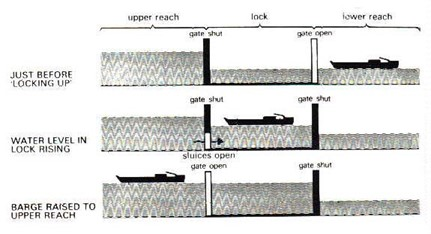
\includegraphics[scale=0.65]{sluismodel.jpg}

\subsubsection{Onderdelen}
Op basis van de schets kunnen we vaststellen dat een sluismodel uit de volgende onderdelen bestaat.

\begin{enumerate}
	\item Een tweetal sluisdeuren. 
	\item Een sluiskolk waarin de schepen in- enuitvaren
	\item een stoplicht om een signaal af te geven voor invaren en uitvaren.
	\item Een nivelleermachine zorgt ervoor dat het water in de sluis op het gewenste niveau wordt gebracht
	\item Een control-system dat ervoor zorgt dat de opdrachten van de sluisbeheerder (geautomatiseerd) worden uitgevoerd
\end{enumerate}
\subsubsection{Werking}

Een schip komt aanvaren en meld zich aan bij de sluismeester. De sluismeester geeft een signaal aan het controlsystem voor het openen van de sluisdeuren, nadat geccontroleerd is of de nivelleermachine al klaar is. Als er ruimte is voor een invarend schip mag het schip dat zoich heeft aangemeld en toestemming heeft  in de sluis varen. Op het moment dat de sluis vol is gaan de sluisdeuren dicht. Eenmaal afgesloten kan de nivelleermachine beginnen om het water in de sluiskolk op het gewenste waterpeil te brengen. Als dit nivelleerprces is afgerond geeft  het controlsystem daan da de sleusdeuren open kunnen.  Als de sleusdeuren open zijn en het uitvaarsignaal is op groen dan moet het schip in de sluis de sluis uitvaren.
\paragraph{extra cases}
Uit het zojuist genoemnde scenario valt het volgende op te maken.
\begin{enumerate}
	\item Een schip geeft een signaal aan een sluismeester.
	\item Er wordt gekeken of er wel plek is in de sluis .
	\item Er wordt gekeken of de nivelleermachine is afgerond.
	\item Er wordt gekeken wat het niveo van de waterpeil in de sluiskolk is.
	\item Er wordt gekeken of de sluisdeuren gereed zijn voor invarende schepen.
\end{enumerate}
\paragraph{Aandachtspunten}
\begin{enumerate}
	\item Voorrang tussen schepen onderling in de sluis?
	\item Hoe lang mag een schip zich in de sluis bevinden?
\end{enumerate} 

%%%%%%%%%%%%%%%%%%%%%%%%%%%%%%%%%%%%%%%%%%%%%%%%%%%%%%%%%%%%%%%%%
\section{Concept}

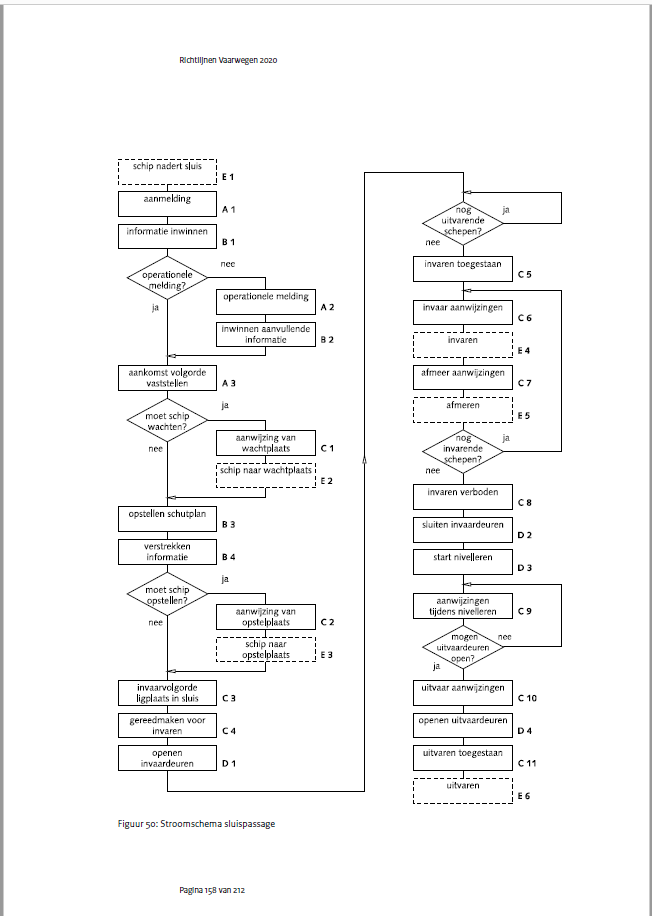
\includegraphics[scale=0.65]{sluispassage.png}

\paragraph{Vooraanmelding}


\paragraph{informatie inwinnen}


\paragraph{operationele melding}


\paragraph{aankomst volgorde}

\paragraph{aanwijzen wachtplaats}


\paragraph{verstrekken informatie}


\paragraph{aanwijzen opstelplaats}

\paragraph{opstellen schutproces}


\paragraph{verstrekken informatie}


\paragraph{invaarvolgorde en ligplaats in sluis}

\paragraph{gereedmaken voor invaren}



\paragraph{openen invaardeuren}




\paragraph{invaren toegestaan}

\paragraph{aanwijzingen voor invaren}
\paragraph{aanwijzingen tijdens afmeren}

\paragraph{invaren verboden}

\paragraph{sluiten invaardeuren}

\paragraph{start nivelleren}

\paragraph{aanzwijzingen voor uitvaren}
\paragraph{openen uitvaardewuren}

\paragraph{uitvaren toegestaan}




\paragraph{brainstorm 22-5-2022}

\subparagraph{invaardeuren en uitvaardeuren}
Gaan we uit van binnendeuren en buitendeuren? Er ontstaat dan een extra ruimte in de sluis. Hoeveel schepen kunnen in deze ruimte? Wat is de maximale wachtreij in deze ruimte en wat zijn de verkeersregels in deze nruimte?
\subparagraph{invaarstoplicht en uitvaarstoplicht}
Als invaren is toegestaan hoe wordt dit dan doorgegeven aan de schepen in de sluis? moeten zij dan uit zichzelf wachten of krijgen zij een signaal dat zij wewl/niet mogen uitvaren? En moeten zij dan kiezen voor links, midden of rechts? Of maakt dat allemaal niets uit?

\subparagraph{invaarwachtrij en uitvaarwachtrij}
Als er meerder schepen in een sluiskolk zitten moet het systeem dan rekeneing houden met het schip dat als eerste is ingevaren en/of het langst in de sluis zit?


%%%%%%%%%%%%%%%%%%%%%%%%%%%%%%%%%%%%%%%%%%%%%%%%%%%%%%%%%%%%%%%%%



\chapter{Kripke model}

\section{Uppaal kripke structuren}


\subsubsection{templates}

\paragraph{Schip}

\paragraph{Sluis}


\paragraph{Aanvoer}


\paragraph{Afvoer}

\paragraph{Pomp}

\paragraph{Pompbediening}


\paragraph{Stoplicht}

\paragraph{Deur}


\subparagraph{case}
Als een schip van rechts binnen komt en sluisdeuren zijn dicht dan moet het stoplicht op rood, de pomnp in transitie van laag naar hoog en niet andersom

\subparagraph{case}
Voor invaren geldt altijd: waterlevel, pomp uit, sluisdeuren open en stoplicht op groen

\subparagraph{case}
uitvarenden hebben voorang op invarenden

\subparagraph{case}
Voor invarenden geldt pomp uit, sleusdeur open en stoplicht op groen
\subparagraph{case}
voor nivelleren geldt pomp is aan, sluisduren zijn doicht en het stoplicht is op rood
\subparagraph{case}
Als een schip vertrekt dan zijn altijd, sleusdeuren open, waterlevel gereed op niveau 5 of 0 en stoplicht direct op groen
\subparagraph{case}
urgent locations; het is niet mogelijk om hier te wachten
\subparagraph{case}
urgent syn; een synchronisatie moet direct worden uitgevoerd als de guards geldig zijn

\subparagraph{case}
als een schip binnen is, en er zijn wachtende schepen, dan moet het stoplicht via oranje naar rood
\subparagraph{case}
committed; als deze staat actief is dan wordt de eerst volgende transitie uitaande van deze state
\subparagraph{case}
als een schjip binnen vaart mnoiet hij ook eft binnen zijn en niet binnenvaren, dit geldt ook voor sluisdeuren en pompen dus deze zijn committed.
\subparagraph{case}

\subparagraph{case}

\subparagraph{case}

\paragraph{Parallele compositie}


\paragraph{Parallele compositie}

\subsubsection{Modeleigenschappel}
\paragraph{Parallele compositie}
Om een sluispark te kunnen modelleren meerdere templates die de verschillende abstracties van het systeem aantonen.

\paragraph{Synchronisatgie}
Zorgt ervoor dat  een transitie die genomen worden in de ene kripke tructuur op hetzelfde moment wordt opgenomen in een andere kripke structuur.
\chapter{CTL logica}


\section{Doel van de test}
\subsection{Wat wordt getest en hoe}


\subsection{toetsen met queries}





\subsection{Operator: AG}
Voor alle paden


\subsection{Operator: EG}
Uiteindelijk geldt er een pad waarvoor geldt

\subsection{Operator: AF}
Voor alle paden/richtingen vroeg of laat
\subsection{Operator: EF}
Er is een pad
\subsection{Operator: AX}
Alle opvolgende toestanden

~\cite{locke_2020}
\subsection{Operator: EX}
Er bestaat vanaf de volgende minstens 1 state waarvoor geldt
\subsection{Operator: p U q}
Er geldt p tot q
~\cite{gnsguides}
\subsection{Operator: p R q}
q moet waar zijn totdat en inclusief de situatie dat p voor het eerst waar is, als p niet geldig is, dan moet q vooraltjd geldig zijn

\chapter{Testresultaten CTL logica}




\begin{center}
	\begin{tabular}{| l | c || r | }
		\hline
		1 &A[] !deadlock  &  TRUE \\ \hline
		2 & A[] not (Sluis.Tussenstop5 \&\& Deur.Klaar\_voor\_uitvaart)  &  Disconnected \\ \hline
		3 & A[]  (Sluis.Voorbereiden imply Deur.Dicht)   &  TRUE\\   \hline
		4 &A[]  (Deur.Dicht imply Counter==0)   & TRUE  \\   \hline
		5 & A[]  (Buitenstoplicht.Groen imply invaren\_allowed==true)  &  TRUE \\ \hline
		6 & A[] ! (Binnenstoplicht.Groen imply invaren\_allowed==false)  & FALSE \\ \hline
		7 & A[]  (globale\_tijd>30)   &  FALSE\\    \hline
		8 & E<>  (Schip.Stoppen and (Counter >5))   & Ship not a structure  \\   \hline
		9 & A[] (Schip.Vertrekken imply Sluisdeur.Dicht)  &  -  \\   \hline
		\hline
	\end{tabular}
\end{center}


 
%  https://www.stat.cmu.edu/~brian/latex/symbols/symbols.html
% https://tex.loria.fr/ctan-doc/macros/latex/doc/html/fntguide/node18.html
% https://observablehq.com/@s-haensch/latex-notation
% http://tdc-www.harvard.edu/tdcprop1/help/symbols/
% http://new.math.uiuc.edu/oldnew/netgeom/advice/to-texpad.html
% https://www.overleaf.com/learn/latex/List_of_Greek_letters_and_math_symbols
% https://jblevins.org/log/greek
% https://latex-tutorial.com/symbols/greek-alphabet/
% https://latex-programming.fandom.com/wiki/List_of_LaTeX_symbols
% https://physicsanduniverse.com/latex-symbols-and-using-them-to-write-equations/
% http://tug.ctan.org/info/symbols/comprehensive/symbols-a4.pdf
% https://tex.stackexchange.com/questions/99772/how-to-insert-greek-letters-having-trouble-with-greekletter
% https://texblog.org/2012/03/15/greek-letters-in-text-without-changing-to-math-mode/
% https://www.avantixlearning.ca/microsoft-word/how-to-insert-greek-letters-or-symbols-in-microsoft-word/
%
%
%








 
\paragraph{resultaat}


%	\bankstatement[title={Kontoauszug 12/2014},
%	openingbalance={-12,34},
%	closingbalance={82,13}]{201412.csv}
 
 
 
 
\subparagraph{verklareing}


\begin{filecontents*}{mydata.csv}
	1.8233,1.8233,1.8233,0.9243,0.8651,0.9013,0.3217,0.3377,34.4858
	0.2753,0.2753,0.2753,0.5383,0.5038,0.5249,0.3217,0.3377,8.4552
	0.0898,0.0898,0.0898,0.2804,0.2625,0.2734,0.3217,0.3377,1.5514
	0.4689,0.1193,0.0417,0.8046,0.2227,0.1795,0.6413,0.3307,6.4488
	0.339,0.8068,0.0936,0.4335,0.8036,0.2434,0.3046,0.624,20.8422
	0.2162,0.133,0.8711,0.1707,0.1503,0.8215,0.1562,0.0692,2.3365
	0.5187,0.9138,1.0432,0.4332,0.8028,0.8406,0.2269,0.3404,22.8164
	0.58,0.2096,0.9086,0.808,0.2134,0.8294,0.333,0.1596,8.4349
	0.8237,0.9378,0.0855,0.8654,0.8096,0.2487,0.4338,0.5187,26.9923 
\end{filecontents*}

\subsection{Fairness}
AG(AF(p))
\begin{verbatim}
	In welke staat de automaat zich ook bevindt, in alle richtingen kom je vroeg of laat een state tegen, waarin p geldig is.
\end{verbatim}
\subsection{Liveness}
\begin{verbatim}
	Altijd en overal geldt: Als p geldt dan geldt vroeg of laat q
	Ookal treedt p nooit p volgens de logica klopt het dan dat q volgt uit p.
	In een situatie, waarin p nooit optreedt, spreekt men van een
	vacuous truth.
\end{verbatim}

 
\VerbatimInput{mydata.csv}

\subsection{safety}
%\VerbatimInput{mydata.txt}

\subsection{zeno vrij}
Geen enkele state kan oneindig een transitie uitvoeren. Elke state heeft een uitgaande transitie.

\subsection{deadlocks}
%\VerbatimInput{data.txt}
 






%	\cleardoublepage
%	
%	% -------------------------------------
%	% CHAPTER 3: IMPORTANT DETAILS
%	% -------------------------------------
%	\chapter{Conclusions}
\label{chapter:Conclusions}
\thispagestyle{myheadings}

% set this to the location of the figures for this chapter. it may
% also want to be ../Figures/2_Body/ or something. make sure that
% it has a trailing directory separator (i.e., '/')!
\graphicspath{{4_Conclusion/Figures/}}


\section{Conclusies}

%\section{Summary of the thesis}
\section{Eindvverantwoording}

Ik heb erg veel geleerd van het analyseren van de vershillende requirements en specificaties en het opzetten van een model in Uppaal. Een dergelijk model opzetten had ik namelijk nog nooit gedaan. Het uitvoeren van onderzoek heb ik eerder gedaan. Ook de toetsing van het model met behulp van proposities heb ik nog nooit gedaan. Verder heb ik de kennis die had van programmeren/ design pattersn gebruikt om de verschillende templates in mijn Uppaal model van elkaar te onderscheiden. Het leukste onderdeel van het project vond ik hoe mijn templatemodel deadlockvrij werkte. Voor de verificatie van het model heb ik veel achtergrondinformatie opgezet, en het is mooi om te zien dat je met enkele duidelijke zinnen kan aantonen of een propositie geldig is of niet.  Verder had ik moeite met het opstellen van de juiste veiligheidseisen bij het model. Ik had aangenomen dat ik het project niet zou halen omdat ik de opdracht niet in teamverband heb uitgevoerd. Ik ben toch blij dat ik een concept heb opgeleverd dat ik kan toetsen aan de doormijzef opgestelde eisen en dat ik met mijn huidige kennis de proposities uit de requirements kan toetsen.



{\bf Important}: In the list of references at the end of thesis, abbreviated journal and conference titles aren't allowed. Either you must put the full title in each item, or create a List of Abbreviations at the beginning of the references, with the abbreviations in one column on the left (arranged in alphabetical order), and the corresponding full title in a second column on the right.  Some abbreviations, such as IEEE, SIGMOD, ACM, have become standardized and accepted by librarians, so those should not be spelled out in full.




\chapter{Discussie}

\subsection{Future work}
\subsubsection{Hoogte waterniveau}

\subsubsection{type deuren naar waterniveau}
De sluis kan ook rekening houden met waterniveau van hoog naar laag.
Als een schip naar binnen vaart moet de sluis weten welk schip ook werer naar buiten vaart en aan welke kant.

\subsubsection{voorrang uitvarend op invarend}
Als een schip uitvaart komt er een moment dat een sluis ruimte vrij heeft. Voordat de sluisdeur sluit nadat eenschip is vertrokken kan er nog een polling worden gedaan naar alle schepen in de buurt om te zien of deze willen en kunnen invaren.

\subsubsection{stoplicht invarend en stoplicht uitvarend}
Een handige functionaliteit is dat voor invarende schepen er een stoplicht is en voor uitvarende schepen. Anders ontstaat er een probleem van collission. 

\subsubsection{Volgorde}
Kunnen aantonen dat schepen kunnen worden behandeld met voorkeur, wie het eerst komt die het eerste in behandeling wordt genomen.	
%	\cleardoublepage
%	
%	% -------------------------------------
%	% CHAPTER 4: CONCLUSIONS
%	% -------------------------------------
%
%		\chapter{Important Details}
\label{chapter:Details}
\thispagestyle{myheadings}

% set this to the location of the figures for this chapter. it may
% also want to be ../Figures/2_Body/ or something. make sure that
% it has a trailing directory separator (i.e., '/')!
\graphicspath{{3_Details/Figures/}}
%
%The use of Type 1 fonts and font embedding into the document are both dependent on a specific Latex installation and even on operating system. There is a good chance that it will work with no problem for you. However, should your thesis PDF be returned, please consider the following remedies discovered by students over many years. 
%
%\section{Type 1 fonts}
%
%All Boston University thesis and dissertation submissions must use only Type 1 fonts to assure high-quality rendering. Type 3 fonts are not acceptable.
%
%For some students adding the following two lines in ``thesis.tex'' preamble has worked:\\
%%
%{\tt
%$\backslash$usepackage[T1]\{fontenc\}\\
%$\backslash$usepackage{pslatex}
%   } 
%
%
%The easiest way to check if fonts are embedded well and of what type, is to use Adobe Acrobat's Preflight -- it shows exactly where the Type 3 fonts are in the thesis. You can learn more here: \url{https://community.adobe.com/t5/acrobat/figure-out-where-a-specific-font-is-used-in-a-pdf/m-p/10880057?page=1#M238035}
%
%If you don't have Adobe Acrobat (BU students get it for free), you can quickly check which fonts have which type by looking into Files $>>$ Properties $>>$ Fonts, but it doesn't tell where the text with a specific font type is.
%
%{\bf Linux/Unix}: If you are using LaTeX or Unix, the problem is that, by default, LaTeX uses Type 3 fonts. Since most users have a tendency to use the default settings, then Type 3 fonts will be used by default. You can try to change the first line in the preamble in ``thesis.tex'' to:\\
%%
%{\tt $\backslash$documentstyle[12pt,times,letterpaper]\{report\}}
%
%\noindent
%since then Times fonts will be used (which are not Type 3). If there are mathematical formulas in the text, it is better to use:\\
%%
%{\tt $\backslash$documentstyle[12pt,times,mathptm,letterpaper]\{report\}}
%
%
%\section{Font embedding}
%
%All fonts must be embedded into the final PDF file. If they are not, sometimes equations may look strange or may not show up at all for several pages. This is often due to unembedded font problem. Should you have a font-embedding issue, this page may prove useful:\\
%%
%\url{https://www.karlrupp.net/2016/01/embed-all-fonts-in-pdfs-latex-pdflatex}
%
%For those using Overleaf, this page might help:
%\url{https://www.overleaf.com/learn/latex/Questions/My_submission_was_rejected_by_the_journal_because_%22Font_XYZ_is_not_embedded%22._What_can_I_do%3F}

%	\cleardoublepage
%	
%	%\appendix
%	\begin{appendices}
%		


\section{Research case: De digitale aanval op de Oekrainese krachtcentrale}
Dit verslag geeft inzage in een analyse van de Ukraine cyber aanval,
inclusief hoe de actoren zich zelf toegang gavan tot het controle systeem, welke methoden de acoren hebben gebruikt voor reconnaissance en vastleggen van het systeem, een gedetailleerde omshrijving van de aanval op 15 December 2015, en de methoden die gebruikt zijn door de aanvallers om hun sporen uit te wissen en daarmee het het stoppen van schade toebrengen  nog moeilker maken. Daarnaast wordter  een gedetailleerde omschrijving gevevenv an de beveiliging van de SCADA ccontrol systemen gebaeerd op bst practices, inclusief het control network ontwerp, technieken voor whtelisting, monitoring en loggen, en  opleiding van personeel.

https://na.eventscloud.com/file_uploads/aed4bc20e84d2839b83c18bcba7e2876_Owens1.pdf
https://www.wired.com/2016/03/inside-cunning-unprecedented-hack-ukraines-power-grid/
https://www.boozallen.com/content/dam/boozallen/documents/2016/09/ukraine-report-when-the-lights-went-out.pdf
https://www.reuters.com/article/us-ukraine-cybersecurity-sandworm-idUSKBN0UM00N20160108
https://www.mandiant.com/resources/blog/ukraine-and-sandworm-team
https://www.ifri.org/sites/default/files/atoms/files/desarnaud_cyber_attacks_energy_infrastructures_2017_2.pdf
https://ris.utwente.nl/ws/files/6028066/3-s2_0-B9780128015957000227.pdf
https://repositorio-aberto.up.pt/bitstream/10216/119066/2/315683.pdf
https://www.diva-portal.org/smash/get/diva2:1046339/FULLTEXT01.pdf
https://www.vice.com/en/article/zmeyg8/ukraine-power-grid-malware-crashoverride-industroyer



Oop 23,december 2015  vind er een cyber aanval plaats op het elektriciteitsnet van de Oekraine. Dit was de eerste bekende aanval op een elektrisch controle  system met corrupte firmware. Daarnaas wordt er een telecom-based denial of service attack met  geautomatieerde systemen om het telefoonverkeer uit te schakelen.
\cite{Whitehead2017ukrainepoweroutage}

Uit onderzoek\cite{zetter2016GridHack} naar de aanval,  uitgevoerd door Oekraiene sen Amerikaanse militairenblijkt  bleek onder meer dat de power grids in sommige gevallen beter waren beveiligd dan de Amerikaanse. Desondanks was de viligheid niet optimaal door onder andere de  hetgegeven dat werknemers op afstand konden inloggen en geen gebruik van 2-stapsverificatie.


\subsection{Literaire analyse}

\subsubsection{Motief}
Oekraine wijst naar de russen \cite{zetter2016GridHack}
https://www.wired.com/story/russian-hackers-attack-ukraine/
https://www.boozallen.com/content/dam/boozallen/documents/2016/09/ukraine-report-when-the-lights-went-out.pdf
https://www.reuters.com/article/us-ukraine-cybersecurity-sandworm/u-s-firm-blames-russian-sandworm-hackers-for-ukraine-outage-idUSKBN0UM00N20160108
https://www.reuters.com/article/us-ukraine-crisis-cyber-idUSKBN15U2CN
https://theconversation.com/cyberattack-on-ukraine-grid-heres-how-it-worked-and-perhaps-why-it-was-done-52802
https://jsis.washington.edu/news/cyberattack-critical-infrastructure-russia-ukrainian-power-grid-attacks/
\subsubsection{Situatie Oekraiene}
https://www.dragos.com/wp-content/uploads/CrashOverride-01.pdf
https://www.dragos.com/wp-content/uploads/CRASHOVERRIDE.pdf
\subsubsection{Situatie algemeen}
https://www.politico.eu/article/ukraine-cyber-war-frontline-russia-malware-attacks/
https://www.ifri.org/sites/default/files/atoms/files/desarnaud_cyber_attacks_energy_infrastructures_2017_2.pdf
https://www.cybersecurityintelligence.com/blog/attack-on-ukraines-power-grid-targeted-transmission-stations-4530.html

\subsubsection{Factoren}
http://web.mit.edu/smadnick/www/wp/2016-22.pdf
\subsubsection{Oorzaak}
https://www.sans.org/blog/confirmation-of-a-coordinated-attack-on-the-ukrainian-power-grid/
https://arstechnica.com/information-technology/2017/06/crash-override-malware-may-sabotage-electric-grids-but-its-no-stuxnet/
https://www.darkreading.com/threat-intelligence/first-malware-designed-solely-for-electric-grids-caused-2016-ukraine-outage
https://www.dragos.com/wp-content/uploads/CRASHOVERRIDE.pdf
\subsubsection{Gebruikte materialen}
https://en.wikipedia.org/wiki/2015_Ukraine_power_grid_hack
https://www.cisa.gov/news-events/alerts/2017/06/12/crashoverride-malware
https://rhebo.com/en/service/glossar/industroyer-25114/


\subsubsection{Uitvoering van de aanval}
https://na.eventscloud.com/file_uploads/aed4bc20e84d2839b83c18bcba7e2876_Owens1.pdf
https://www.boozallen.com/content/dam/boozallen/documents/2016/09/ukraine-report-when-the-lights-went-out.pdf
\subsubsection{Oplossingen}
https://na.eventscloud.com/file_uploads/aed4bc20e84d2839b83c18bcba7e2876_Owens1.pdf
https://www.cisa.gov/news-events/ics-alerts/ir-alert-h-16-056-01
\subsubsection{Aanbevelingen}

\subsection{Resultaten}
\subsubsection{De aanval}
1. An initial email spear phishing attack lures recipients
into opening an attached Microsoft® document with a
macro that installs Black Energy 3 (BE3) onto
corporate workstations.
2. BE3 and other tools perform reconnaissance and
enumeration of the network and provide an initial
backdoor for the hackers into the corporate network.
3. As a result of network reconnaissance, the malicious
actors discover and access the oblenergos’ Microsoft
Active Directory® servers that contain corporate user
accounts and credentials.
4. With the harvested credentials, the malicious actors use
an encrypted tunnel from an external network to get
inside the oblenergo network, establishing a presence
on the oblenergo control system networks.
5. Malicious actors discover and access the control center
supervisory control and data acquisition (SCADA)
human-machine interface (HMI) servers and
substations. While a router separates corporate and
SCADA networks, the firewall rules are improperly
configured.
6. On December 23, 2015, at 3:30 p.m., the malicious
actors begin their power outage attacks by entering
operations and SCADA networks through backdoors on
the compromised SCADA workstations. The malicious
actors take control away from HMI operators and then
open breakers.
7. The malicious actors perform several other actions with
the intent of complicating the responses of control
operators and increasing the effort required to return the
system to normal operating conditions. These actions
include:
a. Launching a coordinated Telephony Denial of
Service (TDoS) attack that floods call centers to
prevent legitimate calls from getting through.
b. Disabling the UPSs for the control centers.
c. Corrupting the firmware on a remote terminal unit
(RTU) HMI module and serial-to-Ethernet port
servers.
8. Malicious actors execute KillDisk malware in an
attempt to wipe out the control center HMIs and pivotpoint workstations.
https://na.eventscloud.com/file_uploads/aed4bc20e84d2839b83c18bcba7e2876_Owens1.pdf
https://www.boozallen.com/content/dam/boozallen/documents/2016/09/ukraine-report-when-the-lights-went-out.pdf
\subsubsection{spearfishing}
\subsubsection{blackenergy}
\subsubsection{remote access capabilities}
\subsubsection{serial-to-ethernet communication devices}
\subsubsection{telephony denial of service attacks}

\subsection{oplossingen}
Identificeer alle risicos en schrijf een plan foor het managen van de risico's.
Implementeer  effecteve controle  om het riico te managen.
Creeer een diepgaand model dat ervoor zor dat er efectieve en efficiente security controls worden uitgevoerd.
Aangaande de gebeurtenissen in de oekraiene kunnen de volgende security controls worden opgenomen in het securitymodel: Initial access to enterprise network, pivot in interprise network, elevate priviliges, maintainance access, gain access to control system, attack, attack complication, destroy hard drives.
\cite{Whitehead2017ukrainepoweroutage}

\subsection{Discussie}

\subsection{Verder lezen}
https://citeseerx.ist.psu.edu/viewdoc/download;jsessionid=0513EED48102FDAD1BD940260EF12B11?doi=10.1.1.548.7490&amp;rep=rep1&amp;type=pdf
https://scialert.net/fulltext/?doi=tasr.2014.396.405
https://www.researchgate.net/publication/333671061_Attacking_IEC-60870-5-104_SCADA_Systems
https://www.welivesecurity.com/wp-content/uploads/2017/06/Win32_Industroyer.pdf
https://blog.nettedautomation.com/2017/
https://arxiv.org/pdf/2001.02925.pdf
https://dl.acm.org/doi/fullHtml/10.1145/3381038
https://www.win.tue.nl/~setalle/2017_fauri_encryption.pdf
http://www.connectivity4ir.co.uk/article/175490/IEC-62351--Secure-communication-in-the-energy-industry.aspx
https://www.virsec.com/resources/blog/virsec-hack-analysis-deep-dive-into-industroyer-aka-crash-override
https://dreamlab.net/en/blog/post/fuzzing-ics-protocols/
https://www.blackhat.com/docs/us-17/wednesday/us-17-Staggs-Adventures-In-Attacking-Wind-Farm-Control-Networks.pdf
https://blog.checkpoint.com/research/crashoverride/
https://www.blackhat.com/us-17/briefings/schedule/#industroyercrashoverride-zero-things-cool-about-a-threat-group-targeting-the-power-grid-6159
https://search.abb.com/library/Download.aspx?DocumentID=9AKK107045A1003&amp;LanguageCode=en&amp;DocumentPartId=&amp;Action=Launch
https://iiot-world.com/ics-security/cybersecurity/five-cybersecurity-experts-about-crashoverride-malware-main-dangers-and-lessons-for-iiot/
https://www.csoonline.com/article/3200828/crash-override-malware-that-took-down-a-power-grid-may-have-been-a-test-run.html
https://www.paloaltonetworks.com/blog/2017/06/crashoverrideindustroyer-protections-palo-alto-networks-customers/
https://www.webopedia.com/definitions/crashoverride-industroyer-malware/
https://www.cyber.nj.gov/threat-center/threat-profiles/ics-malware-variants/crashoverride
https://www.nixu.com/blog/crashoverride-threat-electricity-networks
https://www.virusbulletin.com/virusbulletin/2019/03/vb2018-paper-anatomy-attack-detecting-and-defeating-crashoverride/
https://en.wikipedia.org/wiki/Crash_Override_Network
https://en.wikipedia.org/wiki/Industroyer
https://www.dragos.com/resource/crashoverride-analyzing-the-malware-that-attacks-power-grids/
https://www.wallix.com/blog/ics-security-russian-hacking
https://www.nixu.com/fi/node/53
https://control.com/forums/threads/comparison-between-iec60870-5-103-and-modbus-rtu.20317/





\usepackage{pgf}
%\newcommand\setform{\pgfqkeys{/form }}
%\setform{field1/.store in=\fieldi,
	%	field2/.store in=\fieldii,
	%}


%\addtolength{\oddsidemargin}{-.875in}
%\addtolength{\evensidemargin}{-.875in}
%\addtolength{\textwidth}{1.75in}

%\addtolength{\topmargin}{-.875in}
%\addtolength{\textheight}{1.75in}


\newcommand\myform{%
	\fboxrule=0.4pt
	
	
	\fbox{\begin{minipage}{\textwidth}
			\fbox{\begin{minipage}[t][3cm][t]{0.25\textwidth}
					Betrokken partij
			\end{minipage}}%
			\fbox{\begin{minipage}[t][3cm][t]{0.25\textwidth}
					Verantwoordelijk
			\end{minipage}}%
			\fbox{\begin{minipage}[t][3cm][t]{0.44\textwidth}
					datetimestamp here
			\end{minipage}}
			\fbox{\begin{minipage}[t][1cm][t]{0.98\textwidth}
					Korte notitie 
			\end{minipage}}
			
	\end{minipage}}
	
	\fbox{\begin{minipage}{\textwidth}
			
			\fbox{\begin{minipage}[t][3cm][t]{0.98\textwidth}
					test
			\end{minipage}}
	\end{minipage}}
	
	\fbox{\begin{minipage}{\textwidth}
			\fbox{\begin{minipage}[t][10cm][t]{0.98\textwidth}
					Foto incident
			\end{minipage}}%
			
			
	\end{minipage}}
}



\setform{field1 = G. Wales,
	field2 = Mathematics}
\myform


 
 
 
 
 
 
 
 \section{Bijlage: Testcaes en resultaten}
 \subsection{Wat wordt getest en hoe}
 
 
 \subsection{Requirement specification}
  \begin{verbatim}
 Sluis.Draining-->Deuren.laag_open
 Deuren.laag_open-->Stoplicht.Green
 E<> (Ship.ship_can_move&&Stoplicht.Green)
 A[] not (Stoplicht.Green && not (Deuren.hoog_open||Deuren.laag_open||Deuren.stopgaplow1||Deuren.stopgaplow2||Deuren.stopgaphigh1||Deuren.stopgaphigh2))
 A[] not ((Deuren.hoog_open||Deuren.laag_open||Deuren.Opening_laag||Deuren.Opening_hoog||Deuren.Closing_hoog||Deuren.Closing_laag) && (Sluis.Draining||Sluis.Filling||Sluis.draining2||Sluis.Filling2))
 Sensor.Wait-->Sensor.Wait
 Stoplicht.Green-->Stoplicht.Green
 (Deuren.hoog_open||Deuren.laag_open)-->(Deuren.laag_open||Deuren.hoog_open)
 Deuren.laag_open-->Deuren.Closed
 Deuren.hoog_open-->Deuren.Closed
 Deuren.Closed-->Stoplicht.Red
 Ship.ship_can_move-->Deuren.Closed
 Deuren.hoog_open-->Stoplicht.Green
 Ship.ship_can_move-->Stoplicht.Green
 A[] not (Deuren.laag_open && Deuren.hoog_open)
 Ship.ship_can_move-->Ship.ship_can_move
 A[] not (Deuren.laag_open && Sluis.water != Sluis.water_laag)
 A[] not (Deuren.hoog_open && Sluis.water != Sluis.water_hoog)
 A[]not deadlock
  \end{verbatim}
 
 P2 Het is mogelijk dat de sluispomp in een cyclus teveel water heeft gepompt en dat er daardoor water weggepompt dan wel bijgekompt dient te worden.
 E<> main.waterlevel
 P7  Als zich geen errors voordoen bij stoplicht en deur, maar de waterpomp uitvalt:
 a)  a gear switch is gearanteerd after 1055 ms ( not including  1055)  (deleted)
 a') it is impossible  to switch gear in 1055 ms     (deleted)
 b) it is  impossible to switch gear in less than 550 ms (deleted)
 b') it is possible to switch gear at 550 ms (deleted)
 c) it is impossible to switch  gear in  less than 700 ms if the switch is not from/to gear N (deleted)
 c') it is posible to switch gear at 700 ms if the switch is not from/to gear N (deleted)
 p8 When no error occurs, but engine fails to find synchronous speed
 a) a gear switch is guaranteerd in 1205 ms (incuding 1205)
 a') a gear switch is not gearanteerd at less than 1205 ms
 b) it is imposible to switch gear in less than 450 ms
 b') is is possible to switch gear at 450 ms
 c) it is impossible to switch gear in less than 750 ms if the switch is not from/to gear N
 c') it is not possible to switch gear at 750 ms if the switch is not from/to gear N
 p9 Clutch errors
 a)If the clutch is not closed properly (i.e. a timeout occurs) the gearbox  controller will enter the locationCCCloseError with 200 ms   (undefined)
 b)  When the gearbox controller enters location CCloseError, there is always a problem in the clutch with closing the clutch.  (undefined)
 a) If th clutch is not closed properly (ie. a timeout occurs) the gearbox controller will enter the location CCloseError within 200 ms (undefined)
 b) When the gearbox controller enters location CCloseError, there is always a problem in the clutch with closing the clutch. (undefined)
 p10 Gearbox errors  
 a) If the gearbox can not enter a requested gear ( i.e. a tieout occurs) the gearbox controller will enter the location GsetError within 350 ms (undefined)
 b) When the gearbox controller enters location GSetError, there is always a problem in the gearbox with setting the gear. (undefined)
 p11 IF no error occurs in the engine, it is guaranteed to find synchronous speed (undefined)
 p13 When the gear controller has a greater set, torque regulaton is always indicated in the engine (undefined)
  A[]
 p14
 a) Als de deur open is(ongeacht boven of beneden, dan bevind de sluispomp zich in een predefined state (undefined)
 A[] (gate(0).open||gate(1).open) -> (main.pomp_idle || main.pomp2_idle)
 b) Als de deur is gesloten dan bevind de maincontroller zich in een predefined state
 A[] gate.closed -> main.idle
 p15
 
 p16 If engine regulation is on torque, then the clutch is closed (undefined)
 A[](Engine.Torque imply Clutch.closed
 
 p18 Als een schip van rechts binnen komt en sluisdeuren zijn dicht dan moet het stoplicht op rood, de pomp in transitie van laag naar hoog en niet andersom
 A[] !main.direction -> forall (i:id_d) forall (j:id_s) gate(i).closed && stoplight.rood && main.rd_1
 p19 uitvarenden hebben voorang op invarenden
 
 
 A[] main.s6 -> gate(0).open && gate(1).open && stoplight(0).groen && stoplight(1).groen
 
 
 A[] main.s12 ->
 p23 urgent locations; het is niet mogelijk om hier te wachten
 p24 urgent syn; een synchronisatie moet direct worden uitgevoerd als de guards geldig zijn
 
 A[]
 p26 committed; als deze staat actief is dan wordt de eerst volgende transitie uitaande van deze state
 
 A[]
 p28 Een schip komt aanvaren en geeft een signaal aan de sluis. 
 A[]	
 
 p30 Een schip kan pas naar binnenrijden als de sluisdeuren open zijn, het stoplicht is op groen er er zijn minder dan 2 schepen in de sluis. 	
 A[]  main.s6 && schip.varen ->  Queue.list[N-1] <2
 p32 Eenmaal in de sluis zal het schip moeten wachten op de sluis en de pomp. 	
  A[] Queue.list[N-1] == 2 
 p33 Een schip mag alleen uitvaren als de pomp klaar is, de sleusdeuren open. 
  A[] schip.varen && main.s12 || main.s13 -> (!main.rn1 && !main.rn2)
  
 p34 Een sluis ontvang een aankomst signaal van een schip en bestuurt de sluisdeuren en de pomp. 
  A[]
 p35 De sensor is een onderdeel van de sluis en ontvangt signalen van naderende schepen. 
  A[]

  A[]
 p37 Een pomp begint met pompen bij een signaal van de sluis. Een sluis op zijn beurt geeft alleen een signaal aan de pomp als de sleudeuren dichtzijn
  A[] pomp.pomp_active -> main.s6 && forall(i:id_d) gate(i).closed
 p38 Geen deadlock
 p39 Voor geen enkel pad geldt dat als  de deuren gesloten zijn volgens de sluis dat er een deur openstaat om een schip naar buiten te laten.
 A[] not forall(i:id_d) gate.closed ->(main.s12||main.s13)

 A[] main.s6 -> forall(gate(0).closed
  p41 Voor alle paden geld dat als een deur dicht is het aantal schepen in de kade gelijk is aan nul	
 A[]
 p42 Voor geen enkel pad geld dat als het binnenstoplicht op groen staat dat het niet toegestaan in naar binnen te varen
 E<> stoplight(2).groen || stoploght(3).groen -> main.s6
 p43 Voor alle paden geldt dat de globale tijd langer is dan 30 tijdseenheden
 A[] main.s13-> main.processtime>30
 p44 Er is een pad waarvoor geld dat als een schip wilt stoppen dat er meer dan 5 schepen in de sluis zitten.
 E<>
 p45 Voor alle paden geldt als schip vrtrekt is sluisdeur dicht
 A[] 
 
 A[]
 p47 Er is geen pad waarop een schip vertrekt vanuit de rechtersluisdeur en de linkersluisdeur is open en linkeruitaartstoplicht en linkeruitvaartsoplicht opgroen  en nibelleermachine is aan
 E<>
 p48 Er is een pad waarvoor geldt dat linkerslsuisdeuren dicht zijn, rechtersluisdeuren dicht zijn rechteruitvaartstoplicht is rood en rechteruitvaartstoplicht is  rood terwijl eer geen schip in de sluis licht
 E<> 


 A[] not
 
 A[] (main.waterlevel<waterlaag) -> (!pompwaterweg||pompwaterweg==false)
 
 A[]
 
 A[] not main.rn1 || main.rn2 -> gate(0).open && gate(1).open && Queue.list[N-1] == 0 && ((stoplight(0).groen||stoplight(1).groen) ||(stoplight(3).groen &&stoplight(4).groen))
 p54 Het kan gebeuren dat bij pompr het stoplicht op rood staat, het schip in de sluis en deur is dicht, en waterstand gelijk aan waterlaag
 E<> (main.blocked1 || main.blocked2) -> Queue.list[N-1] >0 && gate(0).closed && gate(1).closed && main.waterlevel==main.waterlevel_laag
 
 E<> main.rn1||main.rn2 -> gate(0).closed &&main.waterlevel==waterlaag
 g
 E<> main.rn1||main.rn2 -> main.waterlevel== main.waterlaag
 p57 Voor alle paden gelt dat er een mogelijkheid is dat deur is open/dicht en sluis nivelleert omhoog/omlaag
 A[] gate(0).open && ()main.direction ==0||main.direction==1)
 p58 A[](1>0)
 
 Fainess:
 
 
 Liveness:
 P1 Na in de idle state te komen, zal de sluis uiteindelijk van richting veranderen. (E<> !Main.Direction)
 p20 Voor invarenden geldt pomp uit, sleusdeur open en stoplicht op groen
 p21 voor nivelleren geldt pomp is aan, sluisduren zijn dicht en het stoplicht is op rood
 A[] (main.rn1 || main.rn2) -> forall (i:id_d) forall(j:id_s )gate(i).closed stoplight(j).rood
 p22 Als een schip vertrekt dan zijn altijd, sleusdeur open, waterlevel gereed op niveau 5 of 0 en stoplicht direct op groen
 p25 als een schip binnen is, en er zijn wachtende schepen, dan moet het stoplicht via oranje naar rood
 p27 als een schip binnen vaart moet hij ook echt binnen zijn en niet binnenvaren, dit geldt ook voor  sluisdeuren en pompen dus deze zijn committed.
 p29 Indien er meer dan twee schepen in de sluis zitten dan wordt het ship geplaats in de wachrij. 
 A[]  Queue.list[N-1] == 2 -> (Sluiskolk.list[N]==1 ||Sluiskolk.list[N]==2)
  p36 De sleusdeur voor boven en beneden kunnen beiden open en dicht. De sluisdeur wordt aangestuurd door de sluis. 
  p55 Er is een mogelijkheid  dat vanuit pomp get stoplicht op rood wordt gezet en waterlevel gelijk is aan waterlaag
  p56 Het kan voorkomen dat bij state pompaan het waterniveau gelijk is aan waterlaa
 
 Securtity:
 P4 Als de richting van een schip gelijk is aan N, dan is het waterlevel niet gelijk aan 1-5 of R
 P5 De sluispomp is nooit in positie AAN, wanneer de sluisdeuren open zijn.
 p17Voor invaren geldt altijd: waterlevel, pomp uit, sluisdeuren open en stoplicht op groen
 A[] main.s5 -> main.waterlevel_laag && idle_pomp1 && gate(0).open && gate(1).open && (stoplight(0).green && stoplight(1).green || stoplight(2).green && stoplight(3).green )
 p40 Voor alle paden geld dat als een sluis aan het voorbereiden is, dan zijn alle deuren dicht.
 p46 Voor alle paden geldt als stoplicht op rood sluisdeuren dicht en schip vertrokken dan is de nivelleermachine uit
 p51 Voor alle paden in een pomp geldt dat als water level lager is dan waterlaag pompwaterweg is altijd false
 p52 Voor alle paden geldt dat als water level hoger is dan waterhoog dan is pompwater altjd false
 p53 Het zal nooit gebeuren dat een pomp water toevoegt als deuren open zjn, geen schip in sluis of stoplicht op groen
 
 Performance:
 P3 Het is al binnen 100 ms mogelijk om te achterhalen aan welke kant de sluisdeuren  open moeten.
 P6 In het geval dat er geen errors zijn (in de stoplichten, sluisdeuren) and ideal (wachtrij) scenario,
 a)  dan is een cyclus gegarandeerd binnen 100 ms (including 100 ms) (undefined)
 a') dan is een cyclus niet gegarandeerd binnen 100 ms
 b)  dan is het onmogelijk om van beneden naar boven te varen, of andersom binnen 150 ms
 b') dan is het mogelijk om van beneden naar boven te varen, of andersom binnen 150 ms
 c)  het is onmogelijk om van richting te veranderen in minder dan 400 ms als de pomp al op niveau x is
 c') het is mogelijk om van richting te veranderen in minder dan 400 ms als de pomp al op niveau x is
 p12 Wanneer beide sluisdeuren in state gesloten zijn, dan is de pomp in zijn initiale state of 100 ms verwijderd van zijn initiele state
 p49 EEn stoplich staat altijd op groen als de deuren open staan en de pomp niet bezig is.
 A[] forall(i:id_s) stoplight.groen -> gate(0).open && gate(1).open && (main.pomp1_idle || main.pomp2_idle)
 p50 In geen enkele staat van de sluis behalve tussen de lowergate en uppergate en uppergate en lowergate en de staten AtArrivalLow en AtEnteringHigh is de wachttijd langer dan 5 tijdseenheden
 
 
 \subsection{Operator: AG}
 Voor alle paden
 
 
 \subsection{Operator: EG}
 Uiteindelijk geldt er een pad waarvoor geldt
 
 \subsection{Operator: AF}
 Voor alle paden/richtingen vroeg of laat
 \subsection{Operator: EF}
 Er is een pad
 \subsection{Operator: AX}
 Alle opvolgende toestanden
 
 ~\cite{locke_2020}
 \subsection{Operator: EX}
 Er bestaat vanaf de volgende minstens 1 state waarvoor geldt
 \subsection{Operator: p U q}
 Er geldt p tot q
 ~\cite{gnsguides}
 \subsection{Operator: p R q}
 q moet waar zijn totdat en inclusief de situatie dat p voor het eerst waar is, als p niet geldig is, dan moet q vooraltjd geldig zijn
 
 
 \subsection{De computation tree}
 
 \subsection{Operator: AG}
 
 \subsection{Operator: EG}
 
 
 Voor alle paden geldt dat waterlevel lager is dan niveau van de kant.
 Voor alle paden geldt dat een omp werkzaam is als alle sluisdeuren dicht zijn.
 Vpoor alle paden geldt dat het aantal schepen in de sluis maximaal 2 is.
 Voor alle padedn  geldt dat een schip nooit langer dan 30 seconden in een sluiskolk zit zonder dat het waterpeil is aangepast.
 \subsection{Operator: EG}
 Er bestaat op elk pad een 
 
 \subsection{Operator: AF}
 
 \subsection{Operator: EF}
 r is soms een mogelijkheid dat twee schepen in de sluis een verschillende uitvaarrichting hebben.
 \subsection{Operator: AX}
 
 
 \subsection{Operator: EX}
 
 \subsection{Operator: p U q}
 
 \subsection{Operator: p R q}
 
 
 Voor alle paden geldt dat een schip alleen kan invaren als de sluisdeur aan de andere zijde is gesloten.
 \subsection{Operator: EX}
 Er bestaat geen situatie dat een pomp actief is terwijl er een sluisdeur open staat
 \subsection{Operator: p U q}
 Vanaf aankomst tot uitvaren is de clocktijd lager dan 30 tijdseenheden 
 \subsection{Operator: p R q}
 Vanaf invaren tot en met uitvarenvan een schip en geldig is x lager dan 15 tijdseenheden
 vanaf aanvaren staat een schip maximaal 40 tijdseenheden in de wahtrij,.
 
 \subsection{Operator: AF}
 Er is altijd meerdere
 \subsection{Operator: EF}
 r is soms een mogelijkheid dat twee schepen in de sluis een verschillende uitvaarrichting hebben.
 \subsection{Operator: AX}
 Voor alle paden geldt dat een schip alleen kan invaren als de sluisdeur aan de andere zijde is gesloten.
 \subsection{Operator: EX}
 Er bestaat geen situatie dat een pomp actief is terwijl er een sluisdeur open staat
 \subsection{Operator: p U q}
 Vanaf aankomst tot uitvaren is de clocktijd lager dan 30 tijdseenheden 
 \subsection{Operator: p R q}
 Vanaf invaren tot en met uitvarenvan een schip en geldig is x lager dan 15 tijdseenheden
 vanaf aanvaren staat een schip maximaal 40 tijdseenheden in de wahtrij,.
 
 \subsection{Fairness}
 
 \subsection{Liveness}
 
 
 
 
 \chapter{Testresultaten CTL logica}
 
 
 
 \begin{center}
 	\begin{gather*}
 		D=\Set{x\in\nat}{1\le x\le 100}\\
 		D=\Set[\big]{x\in\nat}{1\le x\le 100}\\
 		D=\Set[\Big]{x\in\nat}{1\le x\le 100}\\
 		D=\Set[\bigg]{x\in\nat}{1\le x\le 100}\\
 		D=\Set[\Bigg]{x\in\nat}{1\le x\le 100}\\
 		D=\Set*{x\in\nat}{1\le x\le \frac{200}{2}}
 	\end{gather*}
 \end{center}
 
 
 
 
 
 $S is a set of finite states$\\
 $S0 \subseteq S is de set van initiele statess$ \\
 $S0 \subseteq S xS  is een transitie relatie die totaal moet zij, dat betekent, dat voor elke state s \in S er een stats is s' \in S zodat R(s,s')$
 $L\stock a$
 
 $\forall x\,\exists y \implies $
 
 $\mtproforall x\,\mtproexists y \cap \subset \in \vee \diamondsuit \dashv \ni \pm$
 
 
 
 \begin{center}
 	\begin{tabular}{| l | c || r | }
 		\hline
 		1 &A[] !deadlock  &  TRUE \\ \hline
 		2 & A[] not (Sluis.Tussenstop5 \&\& Deur.Klaar\_voor\_uitvaart)  &  Disconnected \\ \hline
 		3 & A[]  (Sluis.Voorbereiden imply Deur.Dicht)   &  TRUE\\   \hline
 		4 &A[]  (Deur.Dicht imply Counter==0)   & TRUE  \\   \hline
 		5 & A[]  (Buitenstoplicht.Groen imply invaren\_allowed==true)  &  TRUE \\ \hline
 		6 & A[] ! (Binnenstoplicht.Groen imply invaren\_allowed==false)  & FALSE \\ \hline
 		7 & A[]  (globale\_tijd>30)   &  FALSE\\    \hline
 		8 & E<>  (Schip.Stoppen and (Counter >5))   & Ship not a structure  \\   \hline
 		9 & A[] (Schip.Vertrekken imply Sluisdeur.Dicht)  &  -  \\   \hline
 		\hline
 	\end{tabular}
 \end{center}
 
 
 
 %  https://www.stat.cmu.edu/~brian/latex/symbols/symbols.html
 % https://tex.loria.fr/ctan-doc/macros/latex/doc/html/fntguide/node18.html
 % https://observablehq.com/@s-haensch/latex-notation
 % http://tdc-www.harvard.edu/tdcprop1/help/symbols/
 % http://new.math.uiuc.edu/oldnew/netgeom/advice/to-texpad.html
 % https://www.overleaf.com/learn/latex/List_of_Greek_letters_and_math_symbols
 % https://jblevins.org/log/greek
 % https://latex-tutorial.com/symbols/greek-alphabet/
 % https://latex-programming.fandom.com/wiki/List_of_LaTeX_symbols
 % https://physicsanduniverse.com/latex-symbols-and-using-them-to-write-equations/
 % http://tug.ctan.org/info/symbols/comprehensive/symbols-a4.pdf
 % https://tex.stackexchange.com/questions/99772/how-to-insert-greek-letters-having-trouble-with-greekletter
 % https://texblog.org/2012/03/15/greek-letters-in-text-without-changing-to-math-mode/
 % https://www.avantixlearning.ca/microsoft-word/how-to-insert-greek-letters-or-symbols-in-microsoft-word/
 %
 %
 %
 
 
 
 
 
 
 \chapter{Time bound derivation}
 
 
 \paragraph{Verification results}
 
 
 %	\bankstatement[title={Kontoauszug 12/2014},
 %	openingbalance={-12,34},
 %	closingbalance={82,13}]{201412.csv}
 
 
 
 
 \subparagraph{verklareing}
 
 
 \begin{filecontents*}{mydata.csv}
 	1.8233,1.8233,1.8233,0.9243,0.8651,0.9013,0.3217,0.3377,34.4858
 	0.2753,0.2753,0.2753,0.5383,0.5038,0.5249,0.3217,0.3377,8.4552
 	0.0898,0.0898,0.0898,0.2804,0.2625,0.2734,0.3217,0.3377,1.5514
 	0.4689,0.1193,0.0417,0.8046,0.2227,0.1795,0.6413,0.3307,6.4488
 	0.339,0.8068,0.0936,0.4335,0.8036,0.2434,0.3046,0.624,20.8422
 	0.2162,0.133,0.8711,0.1707,0.1503,0.8215,0.1562,0.0692,2.3365
 	0.5187,0.9138,1.0432,0.4332,0.8028,0.8406,0.2269,0.3404,22.8164
 	0.58,0.2096,0.9086,0.808,0.2134,0.8294,0.333,0.1596,8.4349
 	0.8237,0.9378,0.0855,0.8654,0.8096,0.2487,0.4338,0.5187,26.9923 
 \end{filecontents*}
 
 \subsection{Fairness}
 AG(AF(p))
 \begin{verbatim}
 	In welke staat de automaat zich ook bevindt, in alle richtingen kom je vroeg of laat een state tegen, waarin p geldig is.
 \end{verbatim}
 \subsection{Liveness}
 \begin{verbatim}
 	Altijd en overal geldt: Als p geldt dan geldt vroeg of laat q
 	Ookal treedt p nooit p volgens de logica klopt het dan dat q volgt uit p.
 	In een situatie, waarin p nooit optreedt, spreekt men van een
 	vacuous truth.
 \end{verbatim}
 
 
 \VerbatimInput{mydata.csv}
 
 \subsection{safety}
 %\VerbatimInput{mydata.txt}
 
 \subsection{zeno vrij}
 Geen enkele state kan oneindig een transitie uitvoeren. Elke state heeft een uitgaande transitie.
 
 \subsection{deadlocks}
 %\VerbatimInput{data.txt}
 
 \newpage
 
 \section{\\ Appendix B: Model eerste deelname aan cursus 2020}
 % the \\ insures the section title is centered below the phrase: Appendix B
 

 
 
 
 \begin{verbatim}
 	
 	Queries
 	Sluis.Draining-->Deuren.laag_open
 	Deuren.laag_open-->Stoplicht.Green
 	E<> (Ship.ship_can_move&&Stoplicht.Green)
 	A[] not (Stoplicht.Green && not (Deuren.hoog_open||Deuren.laag_open||Deuren.stopgaplow1||Deuren.stopgaplow2||Deuren.stopgaphigh1||Deuren.stopgaphigh2))
 	A[] not ((Deuren.hoog_open||Deuren.laag_open||Deuren.Opening_laag||Deuren.Opening_hoog||Deuren.Closing_hoog||Deuren.Closing_laag) && (Sluis.Draining||Sluis.Filling||Sluis.draining2||Sluis.Filling2))
 	Sensor.Wait-->Sensor.Wait
 	Stoplicht.Green-->Stoplicht.Green
 	(Deuren.hoog_open||Deuren.laag_open)-->(Deuren.laag_open||Deuren.hoog_open)
 	Deuren.laag_open-->Deuren.Closed
 	Deuren.hoog_open-->Deuren.Closed
 	Deuren.Closed-->Stoplicht.Red
 	Ship.ship_can_move-->Deuren.Closed
 	Deuren.hoog_open-->Stoplicht.Green
 	Ship.ship_can_move-->Stoplicht.Green
 	A[] not (Deuren.laag_open && Deuren.hoog_open)
 	Ship.ship_can_move-->Ship.ship_can_move
 	A[] not (Deuren.laag_open && Sluis.water != Sluis.water_laag)
 	A[] not (Deuren.hoog_open && Sluis.water != Sluis.water_hoog)
 	A[]not deadlock
 	
	
 \end{verbatim}
 
 \newpage
 \section{\\ Appendix B: Model herkansing tweede deelname aan cursus 2020}
 % the \\ insures the section title is centered below the phrase: Appendix B
 

 
 \begin{verbatim}
 	// Place global declarations here.
 	/*
 	Project working
 	
 	AtArrival
 	StoplightRed
 	DoorOpen
 	StoplightGreen
 	Startmove
 	Sensor
 	SchipEntered
 	Doorclosed
 	StoplightRed
 	---------
 	Nivelleer started
 	NIvelleer stopped
 	Waterlevel equilibrium
 	-----------
 	AtLeaving
 	Stoplightred
 	Dooropened
 	Stoplightgreen
 	StartMove
 	Sensor
 	SchipHasLeft
 	Doorclosed
 	StoplightRed
 	
 	
 	Uitleg
 	Als het schip boven is, dan is waterlvel gelijk aan hoog, filling valve is dicht, lower gates zijn gesloten, uppergates zijn open,empty valve is dicht. 
 	Schip is in waterlock, waterlevel is hoog, filling valve is dicht, lower gates gesloten, upper gates gesloten, empty valve is open. 
 	Schip is dan laag, waterlevel gelijk aan laag, filling valve is dicht, lowergates zijn open, uppergates zijn dicht, empty valve is dicht.
 	AtArrivalHigh
 	
 	AtArrivalLow
 	Als schip beneden is dan is waterlevel gelijk aan laag, filling valve is dicht, lower gates zijn open, upper gates zijn dicht, empty valve is open. 
 	Schip is in water lock, waterlevel is laag, flilling valve is open, lower gates zijn gesloten, upper gates zij gesloten, empty valve is dicht,. 
 	Schip is dan hoog, waterlevel is gelijk aan hoog, filling valve is dicht, uppergates zijn open, lowergates zijn dicht, filling valve is dicht
 	
 	
 	*/
 	
 	const int N = 2;         // # trains
 	typedef int[0,N-1] id_t;
 	
 	chan        appr[N], stop[N], leave[N];
 	urgent chan go[N];
 	
 	// waterniveau in in meter van 0 tot 10
 	typedef int[3,10] waterniveau;
 	
 	waterniveau level;
 	
 	
 	//doors
 	chan lower_gate;
 	chan upper_gate;
 	//filling
 	chan emptying_valve;
 	chan filling_valve;
 	bool nivelleer_sessie_bezig;
 	// water level
 	chan high_water_level;
 	chan low_water_level;
 	//sluices
 	chan signal_sluis_low[N];
 	chan signal_sluis_high[N];
 	//
 	chan move[N];
 	//
 	chan groen;
 	chan rood;
 	
 	clock central;
 	
 	\\geef de schip parameter const id_t id
 	// Place local declarations here.
 	clock schip_clock;
 	
 	\\sensor declaraties
 	clock x;
 	
 	
 	
 	\\sluis declaraties
 	
 	const int water_laag=3;
 	const int water_hoog=10;
 	const int water_median=(water_hoog+water_laag)/2;
 	int[water_laag,water_hoog] water=water_median;
 	// level wordt gelijk gezet met temp
 	// temp is gelijk aan waterniveau
 	clock sluis_clock;
 	id_t list[N+1];
 	int[0,N] len;
 	bool contentHigh, contentLow;
 	// Put an element at the end of the queue
 	void enqueue(id_t element)
 	{
 		list[len++] = element;
 	}
 	
 	// Remove the front element of the queue
 	void dequeue()
 	{
 		int i = 0;
 		len -= 1;
 		while (i < len)
 		{
 			list[i] = list[i + 1];
 			i++;
 		}
 		list[i] = 0;
 	}
 	
 	// Returns the front element of the queue
 	id_t front()
 	{
 		return list[0];
 	}
 	
 	// Returns the last element of the queue
 	id_t tail()
 	{
 		return list[len - 1];
 	}
 	
 	
 	
 	\\stoplicht declaraties
 	clock stoplicht_clock;
 	
 	
 	
 	\\pomp declaraties
 	
 	const int water_laag=3;
 	const int water_hoog=10;
 	const int water_median=(water_hoog+water_laag)/2;
 	int[water_laag,water_hoog] water=water_median;
 	clock pomp_clock;
 	// waterniveau van de sensor voor de sluis is gelijk aan level
 	waterniveau depth;
 	
 	
 	
 	// een constraint op een bepaalde variabele
 	bool isForLow()
 	{
 		//	return false;
 		
 		if( level>=3) return true;
 		else return false;
 		
 	}
 	
 	bool isForHigh()
 	{
 		//	return false;
 		
 		if( level>=6) return true;
 		//else if(level>=6) return true;
 		
 		else return false;
 		
 	}
 	
 	
 	
 	//verschillende tijdseenheden voor even en oneven lampnummers
 	
 	
 	
 	
 	
 \end{verbatim}
 
 
 \chapter{Queries}
 \begin{verbatim}
 	
 	
 	
 	Project declaraties
 	//Declarations
 	
 	chan boot_hoog;
 	chan boot_laag;
 	chan changedoor_low;
 	chan changedoor_high;
 	chan ship_moves;
 	chan ship_abletomove;
 	chan changelight;
 	
 	\\Sluis declaraties
 	const int water_laag=0;
 	const int water_hoog=10;
 	const int water_median=(water_hoog+water_laag)/2;
 	int[water_laag,water_hoog] water=water_median;
 	clock x;
 	\\Stoplicht declaraties
 	
 	\\Ship declaraties
 	clock x;
 	\\Sensor declaraties
 	
 	\\Deuren declaraties
 	bool stoplicht_hoog=false;
 	bool stoplicht_laag=false;
 	clock x;
 	
 	
 	\\System declaraties
 	system Deuren,Sensor,Sluis,Ship,Stoplicht;
 	
 	
 	Uitleg
 	Als het schip boven is, dan is waterlvel gelijk aan hoog, filling valve is dicht, lower gates zijn gesloten, uppergates zijn open,empty valve is dicht. 
 	Schip is in waterlock, waterlevel is hoog, filling valve is dicht, lower gates gesloten, upper gates gesloten, empty valve is open. 
 	Schip is dan laag, waterlevel gelijk aan laag, filling valve is dicht, lowergates zijn open, uppergates zijn dicht, empty valve is dicht.
 	AtArrivalHigh
 	
 	AtArrivalLow
 	Als schip beneden is dan is waterlevel gelijk aan laag, filling valve is dicht, lower gates zijn open, upper gates zijn dicht, empty valve is open. 
 	Schip is in water lock, waterlevel is laag, flilling valve is open, lower gates zijn gesloten, upper gates zij gesloten, empty valve is dicht,. 
 	Schip is dan hoog, waterlevel is gelijk aan hoog, filling valve is dicht, uppergates zijn open, lowergates zijn dicht, filling valve is dicht
 	
 	
 	
 \end{verbatim}
 
 
 
 
 \section{Deelonderzoek naar veiligheidsrisico's en eisen voor sluizen}
 
  %%%%%%%%%%%%%%%%%%%%%%%%%%%%%%%%%%%%%%%%%%%%%%%%%%%%%%%%%%%%%%%%%
 \section{Deelonderzoek wet en regelgeving voor sluizen}
 
 
 
 Gevonden weblinks in google op 07-04-2023 met zoekopdracht: "wet en regelgeving voor sluizen"
 
  %%%%%%%%%%%%%%%%%%%%%%%%%%%%%%%%%%%%%%%%%%%%%%%%%%%%%%%%%%%%%%%%%
  
  
  
 \usepackage{pgf}
 \newcommand\setform{\pgfqkeys{/form }}
 \setform{field1/.store in=\fieldi,
 	field2/.store in=\fieldii,
 }
 
 
 %\addtolength{\oddsidemargin}{-.875in}
 %\addtolength{\evensidemargin}{-.875in}
 %\addtolength{\textwidth}{1.75in}
 
 %\addtolength{\topmargin}{-.875in}
 %\addtolength{\textheight}{1.75in}
 
 
 \newcommand\myform{%
 	\fboxrule=0.4pt
 	
 	
 	\fbox{\begin{minipage}{\textwidth}
 			\fbox{\begin{minipage}[t][3cm][t]{0.25\textwidth}
 					Naam vergadering
 			\end{minipage}}%
 			\fbox{\begin{minipage}[t][3cm][t]{0.25\textwidth}
 					Datum en plats
 			\end{minipage}}%
 			\fbox{\begin{minipage}[t][3cm][t]{0.44\textwidth}
 					Namen aanwezigen
 			\end{minipage}}
 			\fbox{\begin{minipage}[t][1cm][t]{0.98\textwidth}
 					Opening en goedkeuring
 			\end{minipage}}
 			
 	\end{minipage}}
 	
 	\fbox{\begin{minipage}{\textwidth}
 			
 			\fbox{\begin{minipage}[t][3cm][t]{0.98\textwidth}
 					Ingekomen stukken en rondvraag
 			\end{minipage}}
 	\end{minipage}}
 	
 	\fbox{\begin{minipage}{\textwidth}
 			\fbox{\begin{minipage}[t][10cm][t]{0.98\textwidth}
 					Sluiting
 			\end{minipage}}%
 			
 			
 	\end{minipage}}
 }
  %%%%%%%%%%%%%%%%%%%%%%%%%%%%%%%%%%%%%%%%%%%%%%%%%%%%%%%%%%%%%%%%%
 
 \newpage
 
 
 
 
 
 
 
 
 \begin{center}  
 	\begin{tabular}{ | l | l | l | p{5cm} |} % you can change the dimension according to the spacing requirements  
 		\hline  
 		\multicolumn{4}{|l|}{Actielijst} \\ \hline  
 		Onderwerp & Besluit & Wie &Gereed \\ \hline  
 		Orange & Fruit & Vitamin C & It is fruit, which is full of nutrients and low in calories. They can promote clear, healthy skin and also lowers the risk for many diseases. It reduces cholesterol and also helps in building a healthy immune system.\\ \hline  
 		
 		Cauliflower & vegetable & B-Vitamins & It is the vegetable, which is high in fiber and B-Vitamins. It also provides antioxidants, which help in fighting or protect against cancer. It enhances digestion and has many other nutrients.\\ \hline  
 		
 	\end{tabular}  
 \end{center}  
 
 
 
 
 \chapter{Testresultaten}
 
 
 
 \subsubsection{onderdeleel van de test}
 
 
 
 \begin{tabular}{*{15}{|l|l|l|l|l|l|l|}} \hline
 	\multicolumn{7}{|l|}{project name}                                                               \\ \hline
 	\multicolumn{4}{|l|}{Test case ID}   &\multicolumn{3}{|l|}{Test designed by}                           \\ \hline
 	\multicolumn{4}{|l|}{test priority (low/medium/high)}   &\multicolumn{3}{|l|}{Test design date}                           \\ \hline
 	\multicolumn{4}{|l|}{Module name}   &\multicolumn{3}{|l|}{Test executed by}                           \\ \hline
 	\multicolumn{4}{|l|}{Test title}   &\multicolumn{3}{|l|}{Test execution date}                           \\ \hline
 	\multicolumn{4}{|l|}{Description}   &\multicolumn{3}{|l|}{ }                           \\ \hline 		
 	\multicolumn{7}{|l|}{ }   																\\ \hline
 	\multicolumn{7}{|l|}{Pre condition}                                                               \\ \hline
 	\multicolumn{7}{|l|}{Dependencies}                                                               \\ \hline
 	\multicolumn{7}{|l|}{ }   															\\ \hline
 	Step  &  Test steps & Test data & expected result &Acual result &(pass or fail)&notes  \\ \hline
 	
 \end{tabular}
 
 
 
 
 
 \section{Modelleren}
 
 
 \section{Ethiek}
 
 
 \section{Conclusie}
 
 
 \chapter{Security}
 
 \section{Inleiding}
 
 \section{Resultaat}
 

%	\end{appendices}
%	%==========================================================================%
%	% Bibliography
%	\newpage
%	\singlespace
%	\bibliographystyle{apalike}
%	
%	% each subdirectory can have its own BiBTeX file
%	\bibliography{thesis}
%	\cleardoublepage
%	
%	%==========================================================================%
%	% Curriculum Vitae
%	\addcontentsline{toc}{chapter}{Mijn profiel}


\begin{center}
{\LARGE {\bf Mijn werkzaamheden}}\\
\vspace{0.5in}
{\large {\bf Galvin Bartes}}
\end{center}

Basically, this needs to be worked out by each individual, however the same format, margins, typeface, and type size must be used as in the rest of the dissertation. 
 
%	
%	%==========================================================================%
%\end{document}